%%%%&latex
\documentclass[12pt]{article}
\usepackage{amsmath}
\usepackage{graphicx}
\usepackage{psfrag,epsf,enumerate}
\usepackage{enumerate}
\usepackage{natbib}
\usepackage{url} % not crucial - just used below for the URL

\usepackage{amssymb, qtree, bm, multirow, textcmds, siunitx,paralist}
\usepackage{mathrsfs, float, booktabs,todonotes,amsthm}
\usepackage[bb=boondox]{mathalfa}
\usepackage{tikz}
\usetikzlibrary{arrows,positioning,shapes,fit,calc}
\usepackage{amsfonts}
\usepackage[section]{placeins}
\usepackage{amsthm,algorithm,algorithmicx,algpseudocode}
%\pdfminorversion=4
% NOTE: To produce blinded version, replace "0" with "1" below.
\newcommand{\blind}{1}

% DON'T change margins - should be 1 inch all around.
\addtolength{\oddsidemargin}{-.5in}%
\addtolength{\evensidemargin}{-.5in}%
\addtolength{\textwidth}{1in}%
\addtolength{\textheight}{1in}%
\addtolength{\topmargin}{-.8in}%

\DeclareMathOperator*{\argmin}{arg\,min}
\newcolumntype{L}{>{$}l<{$}} % math-mode version of "l" column type
\def\mathbi#1{\textit{ #1}}
\def\mathB#1{\textbf{ #1}}
\def\E{\text{E}}
\def\var{\text{Var}}

\def\PQ{\begin{pmatrix}\bm{G}\\[-0.2cm]\bm{G}'_{\perp}\end{pmatrix}}
\def\bt{\begin{pmatrix}{\bm{b}}\\[-0.2cm]{\bm{a}}\end{pmatrix}}

%\theoremstyle{theo}
\newtheorem{theo}{Theorem}[section]

\theoremstyle{definition}
\newtheorem{definition}{Definition}[section]



\begin{document}


	%\bibliographystyle{natbib}
	
	\def\spacingset#1{\renewcommand{\baselinestretch}%
		{#1}\small\normalsize} \spacingset{1}
	
	
	%%%%%%%%%%%%%%%%%%%%%%%%%%%%%%%%%%%%%%%%%%%%%%%%%%%%%%%%%%%%%%%%%%%%%%%%%%%%%%
	
	\if1\blind
	{
		\title{\bf Probabilistic Forecasts for Hierarchical~Time~Series}
		        \author{Puwasala Gamakumara\\
			    Department of Econometrics and Business Statistics,\\
			    Monash University,\\ VIC 3800, Australia.\\
			    Email: puwasala.gamakumara@monash.edu \\
			    and \\
			    Anastasios Panagiotelis\thanks{
			    	The authors gratefully acknowledge the support of Australian Research Council Grant DP140103220.  We also thank Professor Mervyn Silvapulle for valuable comments.}\hspace{.2cm}\\
			    Department of Econometrics and Business Statistics,\\
		    	Monash University,\\ VIC 3800, Australia.\\
			    Email: anastasios.panagiotelis@monash.edu \\
			    and \\
		        George Athanasopoulos\\
		        Department of Econometrics and Business Statistics,\\
		        Monash University,\\ VIC 3800, Australia.\\
		        Email: george.athanasopoulos@monash.edu \\
		        and \\
	            Rob J Hyndman\\
	            Department of Econometrics and Business Statistics,\\
	            Monash University,\\ VIC 3800, Australia.\\
	            Email: rob.hyndman@monash.edu \\}
		\maketitle
	} \fi
	
	\if0\blind
	{
		\bigskip
		\bigskip
		\bigskip
		\begin{center}
			{\LARGE\bf Probabilistic Forecasts for Hierarchical~Time~Series}
		\end{center}
		\medskip
	} \fi
	
	\bigskip


\begin{abstract}
	TBC
%  Forecast reconciliation involves adjusting forecasts to ensure coherence with aggregation constraints. We extend this concept from point forecasts to probabilistic forecasts by redefining forecast reconciliation in terms of linear functions in general, and projections more specifically. New theorems establish that the true predictive distribution can be recovered in the elliptical case by linear reconciliation, and general conditions are derived for when this is a projection. A geometric interpretation is also used to prove two new theoretical results for point forecasting; that reconciliation via projection both preserves unbiasedness and dominates unreconciled forecasts in a mean squared error sense. Strategies for forecast evaluation based on scoring rules are discussed, and it is shown that the popular log score is an improper scoring rule with respect to the class of unreconciled forecasts when the true predictive distribution coheres with aggregation constraints. Finally, evidence from a simulation study shows that reconciliation based on an oblique projection, derived from the MinT method of \citet{Wickramasuriya2017} for point forecasting, outperforms both reconciled and unreconciled alternatives.
\end{abstract}

%\noindent%
%{\it Keywords:}  Forecast Reconciliation, Projections, Elliptical Distributions, Scoring Rules, High-dimensional Time Series.
%\vfill

\newpage
\spacingset{1.45} % DON'T change the spacing!

\section{Introduction}\label{sec:intro_chap3}

Large collections of time series often follow some aggregation structure. For example, tourism flows of a country can be disaggregated along a geographic hierarchy of states, zones, and cities. Such collections of time series are generally referred to as hierarchical time series. To ensure aligned decision making, it is important that forecasts across all levels of aggregation add up. This property is called ``coherence''. If the forecasts are not coherent, then these can be adjusted so that they become coherent. Earlier approaches for obtaining coherent forecasts involve generating first-stage forecasts for series in a single level of the hierarchy and then aggregating these up or disaggregate these down to obtain forecasts for the remaining series. These are often call ``bottom-up'' and ``top-down'' forecasts respectively. For example see \citet{Dunn1976}, \citet{Gross1990} and references therein.

An alternative approach to these single level forecasting methods is to do forecast ``reconciliation''. Reconciliation starts with a set of incoherent forecasts for the entire hierarchy and then revises these so that they are coherent with the aggregate constraints, see for example \citet{AthEtAl2009, HynEtAl2011, VanErven2015a, ShaHyn2017}. From this literature we see that coherency and reconciliation has been extensively developed for the point forecasting case. Generalising both of these concepts, particularly the latter, to probabilistic forecasting is a gap that we seek to address in this chapter.
%We do so by extending the geometric interpretation to coherence and reconciliation in the point forecasting case outlined in Chapter \ref{Chap:ForeRecon} to the probabilistic framework. This allows us to derive further results for parametric as well as non-parametric distributional forecasts for hierarchical time series.
%elliptical distributions as well as provide insight into forecast evaluation via multivariate scoring rules.

%Traditional approaches to ensure coherent point forecasts produce first-stage forecasts at a single level of the hierarchy. To describe these we use the small hierarchy in Figure~\ref{fig1} where the variable labelled $Tot$ is the sum of the series $A$ and series $B$, the series $A$ is the sum of series $AA$ and series $AB$ and the series $B$ is the sum of the series $BA$ and $BB$. In the bottom-up approach \citep{Dunn1976}, forecasts are produced at the most disaggregated level (series $AA$, $AB$, $BA$ and $BB$) and then summed to recover forecasts for all higher-level series. Alternatively, in the top-down approach \citep{Gross1990}, a top-level forecast is first produced (series $Tot$) and bottom-level forecasts are recovered by disaggregating the forecast using either historical or forecasted proportions. A middle-out approach is a hybrid between these two, that for the hierarchy in Figure~\ref{fig1} would produce first stage forecasts for series $A$ and $B$.
%

%
%In recent years, reconciliation methods introduced by \citet{Hyndman2011} have become increasingly popular. For these methods, first stage forecasts are independently produced for all series rather than series at a single level. Since these so-called `base' forecasts are rarely coherent in practice, they are subsequently adjusted or `reconciled' to ensure coherence. Note that we use coherence and reconciliation as distinct terms, in contrast to their at times ambiguous usage in the past. To date, reconciliation has typically been formulated as a regression problem with alternative reconciliation methods resembling different least squares estimators. These include Ordinary Least Squares {OLS} \citep{Hyndman2011}, Weighted Least Squares {WLS} \citep{AthEtAl2017}, and a Generalised Least Squares (GLS) estimator \citep{WicEtAl2019} named MinT since it minimises the trace of the squared error matrix. These methods have been shown to outperform traditional alternatives across a range of simulated and real-world datasets \citep{AthEtAl2009,VanErven2015a,WicEtAl2019} since they use information at all levels of the hierarchy and, in some sense, hedge against the risk of model misspecification at a single level.

% This requirement motivated researchers to find the entire probability distribution of the future values so that it provides a full description of the uncertainty associated with the prediction

In contrast to the point forecasts, the entire probability distribution of future values provides a full description of the uncertainty associated with the predictions \citep{Abramson1995, Gneiting2014}. Therefore probabilistic forecasting has become of great interest in many disciplines such as, economics \citep{zarnowitz1987, rossi2014}, meteorological studies \citep{pinson2009, mclean2013}, energy forecasting \citep{wytock2013, BenTaieb2017} and retail forecasting \citep{bose2017}. However, the attention on probabilistic forecasts in the hierarchical literature has been limited. Indeed to the best of our knowledge, \citet{Taieb2017} and \citet{JeoEtAl2019} are the only papers to deal with probabilistic forecasts in the hierarchical time series. Although \citet{Taieb2017} reconcile the means of predictive distributions, the overall distributions are constructed in a bottom-up fashion rather than using a reconciliation approach. \citet{JeoEtAl2019} propose a novel method for probabilistic forecast reconciliation based on cross-validation which is particularly applied to temporal hierarchies. In contrast to these studies, the main objective of this chapter is to generalise both the concepts of coherence and reconciliation from point to probabilistic forecasting.

%To facilitate the extension of point forecast reconciliation to probabilistic forecasting, we first provide a geometric interpretation of existing point reconciliation methods, framing them in terms of projections. In addition to being highly intuitive, this allows us to establish a number of theoretical results. We prove two new theorems about point forecast reconciliation, the first showing that reconciliation via projections preserves the unbiasedness of base forecasts, while the second shows that reconciled forecasts dominate unreconciled forecasts via the distance reducing property of projections.


Extending the geometric interpretation related to point forecast reconciliation derived in \citep{PanEtAl2019HF} we provide new definitions of coherence and forecast reconciliation in the probabilistic setting. We also cover the topic of forecast evaluation of probabilistic forecasts via scoring rules. In particular, we prove that for a coherent data generating process, the log score is not proper with respect to incoherent forecasts. Therefore we recommend the use of the energy score or variogram score for comparing reconciled to unreconciled forecasts. Two or more reconciled forecasts can be compared using log score, energy score or variogram score, although we show that comparisons should be made on the full hierarchy for the latter two scores.

When parametric density assumptions are made we describe how the probabilistic forecast definitions lead to a reconciliation procedure that merely involves a change of basis and marginalisation. We show that probabilistic reconciliation via linear transformations can recover the true predictive distribution as long as the latter is in the elliptical class. We provide conditions for which this linear transformation is a projection, and although this projection cannot be feasibly estimated in practice, we provide a heuristic argument in favour of MinT reconciliation.

Further we propose a new method to generate coherent forecasts when the parametric distributional assumptions are not applicable. This method uses a non-parametric bootstrap based approach to generate future paths for all series in the hierarchy and then reconcile each sample path using projections. This will provide a possible sample from the reconciled predictive density of the hierarchy. An extensive simulation study was carried out to find the optimal reconciliation of bootstrap future paths with respect to a proper scoring rule. This has shown that the MinT method is at least as good as the optimal method for reconciling future paths.

Finally we applied both parametric and non-parametric approaches to generate probabilistic forecasts for domestic tourism flow in Australia. The results show that reconciliation improves forecast accuracy compared to incoherent forecasts in both parametric and non-parametric approaches and furthermore, MinT reconciliation performs best.

The remainder of the paper is structured as follows. In Section~\ref{sec:Notat&Prelim} notation and some preliminary work on point forecast reconciliation is discussed. Section~\ref{sec:ProbForecasts} contains the definitions and interpretation of coherent probabilistic forecasts and reconciliation. In Section~\ref{sec:evaluation} we consider the evaluation of probabilistic hierarchical forecasts via scoring rules. Parametric forecast reconciliation and some theoretical results related to elliptical distributions are discussed in Section~\ref{sec:ParamRecon} while the non-parametric approach is introduced in Section~\ref{sec:non-para}. An empirical application on tourism forecasting is contained in Section~\ref{sec:Application}. Finally Section~\ref{sec:conclusions_chap3} concludes with some discussion and thoughts on future research.

\section{Hierarchical probabilistic forecasts}\label{sec:ProbForecasts}

Before introducing coherence and reconciliation to the probabilistic setting, we first briefly refresh these concepts in the case of the point forecasts.  In doing so, we follow the geometric interpretation introduced by \cite{PanEtAl2019HF}, since this formulation provides a natural framework for generalisation to probabilistic forecasting.


\subsection{Point Forecasting}\label{sec:Notat&Prelim}

A \emph{hierarchical time series} is a collection of time series adhering to some known linear constraints.  Stacking the value of each series at time $t$ into an $n$-vector ${\bm y}_t$, the constraints imply that ${\bm y}_t$ lies in an $m$-dimensional linear subspace of $\mathbb{R}^n$ for all $t$.  This subspace is referred to as the {\em coherent subspace} and is denoted as $\mathfrak{s}$.  A typical (and the original) motivating example is a collection of time series some of which are aggregates of other series. In this case $\bm{b}_t \in \mathbb{R}^m$ can be defined as the values of the most disaggregated or \emph{bottom-level series} at time $t$ and the aggregation constraints can be formulated as,
\begin{equation*}
\bm{y}_t = \bm{Sb}_t,
\end{equation*}
where $\bm{S}$ is an $n \times m$ constant matrix for a given hierarchical structure.

\begin{figure}[H]
	\begin{center}
		\leaf{AA} \leaf{AB}
		\branch{2}{A}
		\leaf{BA} \leaf{BB}
		\branch{2}{B}
		\branch{2}{Tot}
		\qobitree
	\end{center}
	\caption{An example of a two level hierarchical structure.}\label{fig:twoL-hier}
\end{figure}
An example of a hierarchy is shown in Figure~\ref{fig:twoL-hier}. There are $n=7$ series of which $m=4$ are bottom-level series. Also, $\bm{b}_t = [y_{AA,t}, y_{AB,t}, y_{BA,t}, y_{BB,t}]'$, $\bm{y}_t = [y_{Tot,t},y_{A,t}, y_{B,t},\bm{b}'_t]'$,  and
\[
\bm{S} = \begin{pmatrix}
1 & 1 & 1 & 1 \\
1 & 1 & 0 & 0 \\
0 & 0 & 1 & 1 \\
& \multicolumn{2}{c}{\bm{I}_4} &
\end{pmatrix},
\]
where $\bm{I}_4$ is the $4\times 4$ identity matrix.

The connection between this characterisation and the coherent subspace is that the columns of $\bm{S}$ span $\mathfrak{s}$.  Below, the notation $s:\mathbb{R}^m\rightarrow\mathbb{R}^n$ is used when premultiplication by $\bm{S}$ is though of as a mapping.  Finally, while $\bm{S}$ is defined in terms of $m$ bottom-level series here, in general any $m$ series can be chosen with the $\bm{S}$ matrix redefined accordingly.  The columns of all appropriately defined $\bm{S}$ matrices span the same coherent subspace $\mathfrak{s}$.

When forecasts of all $n$ series are produced, they may not adhere to constraints.

In this case forecasts are called {\em incoherent base} forecasts and are denoted $\hat{\bm y}_{t+h}$, with the subscript $t+h$ implying a $h$-step ahead forecast at time $t$.  To exploit the fact that the target of the forecast adheres to known linear constraints, these forecasts can be adjusted in a process known as {\em forecast reconciliation}.  At its most general, this involves selecting a mapping $\psi:\mathbb{R}^n\rightarrow\mathfrak{s}$ and then setting $\tilde{\bm y}_{t+h}=\psi(\hat{\bm y}_{t+h})$, where $\tilde{\bm y}_{t+h}\in\mathfrak{s}$ is called the {\em reconciled} forecast.  The mapping $\psi$ may be considered as the composition of two mappings $\psi=s\circ g$. Here, $g:\mathbb{R}^{n}\rightarrow\mathbb{R}^{m}$ combines incoherent base forecasts of all series to produce new bottom-level forecasts, which are then aggregated via $s$.  When $g$ is a linear mapping this corresponds to pre-multiplying base forecasts by a matrix $\bm{S}\bm{G}$.

\cite{PanEtAl2019HF} discuss how a number of important properties arise when $\bm{S}\bm{G}$ is a projection matrix.  In this case, ${\bm G}$ can be written as $(\bm{R}_{\perp}'\bm{S})^{-1}\bm{R}_{\perp}'$, where $\bm{R}_{\perp}$ is an $n\times m$ orthogonal complement to the $n\times(n-m)$ matrix $\bm{R}$, with $\bm{R}$ defining a direction of projection.  For instance, OLS reconciliation \citep{HynEtAl2011} projects along a direction perpendicular to $\bm{S}$, in which case $\bm{R}=\bm{S}_{\perp}$, $\bm{R}_{\perp}=\bm{S}$ and $\bm{G}=(\bm{S}'\bm{S})^{-1}\bm{S}'$.  Several other choices of $\bm{G}$ currently extant in the literature, including the bottom-up \citep{Dunn1976} WLS \citep[][]{Hyndman2016,AthEtAl2017} and MinT \citep{WicEtAl2019} methods, are also special cases where $\bm{S}\bm{G}$ is a projection.

\subsection{Coherent probabilistic forecasts}\label{subsec:cohprobf}

We now turn our attention towards a novel definition of coherence in a probabilistic setting.  First let $(\mathbb{R}^m, \mathscr{F}_{\mathbb{R}^m}, \nu)$ be a probability triple, where $\mathscr{F}_{\mathbb{R}^m}$ is the usual Borel $\sigma$-algebra on $\mathbb{R}^m$. This triple can be thought of as a probabilistic forecast for the bottom-level series.  A $\sigma$-algebra $\mathscr{F}_{\mathfrak{s}}$ can then be constructed as the collection of sets $s(\mathcal{B})$ for all $\mathcal{B}\in \mathscr{F}_{\mathbb{R}^m}$, where $s(\mathcal{B})$ denotes the image of $\mathcal{B}$ under the mapping $s$.

\begin{definition}[Coherent Probabilistic Forecasts]\label{def:cohprob}
	Given the triple, $(\mathbb{R}^m, \mathscr{F}_{\mathbb{R}^m}, \nu)$, a coherent probability triple $(\mathfrak{s}, \mathscr{F}_{\mathfrak{s}}, \breve{\nu})$, is given by $\mathfrak{s}$, the sigma algebra $\mathscr{F}_{\mathfrak{s}}$ and a measure $\breve{\nu}$, such that
	\[
	\breve{\nu}(s(\mathcal{B})) = \nu(\mathcal{B}) \quad \forall \mathcal{B} \in \mathscr{F}_{\mathbb{R}^m}.
	\]
\end{definition}

To the best of our knowledge, the only other definition of coherent probabilistic forecasts is given by \citet{BenTaieb2017} who define coherent probabilistic forecasts in terms of convolutions. While these definitions do not contradict one another our definition has two advantages.  First it can more naturally be extended to problems with non-linear constraints with the coherent subspace $\mathfrak{s}$ replaced with a manifold.  Second, the geometric understanding of coherence facilitates a definition of probabilistic forecast reconciliation to which we now turn our attention.

\subsection{Probabilistic forecast reconciliation} \label{subsec:ProbForecastRecon}

Let $(\mathbb{R}^n, \mathscr{F}_{\mathbb{R}^n}, \hat{\nu})$ be a probability triple characterising a probabilistic forecast for all $n$ series. The hat is used for $\hat{\nu}$ analogously with $\hat{\bm y}$ in the point forecasting case.  The objective is to derive a reconciled measure $\tilde{\nu}$, assigning probability to each element of the $\sigma$-algebra $\mathscr{F}_\mathfrak{s}$.

\begin{definition} \label{def:reconprob}
	The reconciled probability measure of $\hat{\nu}$ with respect to the mapping $\psi(.)$ is a probability measure $\tilde{\nu}$ on $\mathfrak{s}$ with $\sigma$-algebra $\mathscr{F}_\mathfrak{s}$ such that
	\[
	\tilde{\nu}(\mathcal{A}) =  \hat{\nu}(\psi^{-1}(\mathcal{A})) \qquad \forall \mathcal{A} \in \mathscr{F}_{\mathfrak{s}}\,,
	\]
	where $\psi^{-1}(\mathcal{A}):=\{{\bm{y}}\in \mathbb{R}^n:\psi({\bm{y}})\in \mathcal{A}\}$ is the pre-image of $\mathcal{A}$, that is the set of all points in $\mathbb{R}^n$ that $\psi(.)$ maps to a point in $\mathcal{A}$.
\end{definition}

This definition naturally extends forecast reconciliation to the probabilistic setting. In the point forecasting case, the reconciled forecast is obtained by passing an incoherent forecast through a transformation. Similarly, for probabilistic forecasts, to determine the probability assigned to a region of points by the reconciled forecast, we consider the probability assigned by the base forecasts to all points mapped to that region by a transformation.  Recall that the mapping $\psi$ can also be expressed as a composition of two transformations $s\circ g$. In this case, an $m$-dimensional reconciled probabilistic distribution $\nu$ can be obtained such that $\nu(\mathcal{B})= \hat{\nu}(g^{-1}(\mathcal{B}))$ for all $\mathcal{B} \in \mathscr{F}_{\mathbb{R}^m}$ and a probabilistic forecast for the full hierarchy can then be obtained via Definition~\ref{def:cohprob}.  This construction will be used in Section~\ref{sec:ParamRecon}.

Defintion~\ref{def:reconprob} can use any continuous mapping $\psi$, where continuity is required to ensure that open sets in $\mathbb{R}^n$ used to construct $\mathscr{F}_{\mathbb{R}^n}$ are mapped to open sets in $\mathfrak{s}$.  However, hereafter, we restrict our attention to $\psi$ as a linear mapping.  This is depicted in Figure~\ref{fig:probfr_sch} when $\psi$ is a projection.  This figure is only a schematic, since even the most trivial hierarchy is $3$-dimensional.  The arrow labelled $\bm{S}$ spans an $m$-dimensional coherent subspace $\mathfrak{s}$, while the arrow labelled $\bm{R}$ spans an $n-m$-dimensional direction of projection.  The mapping $g$ collapses all points in the blue shaded region $g^{-1}(\mathcal{B})$, to the black interval $\mathcal{B}$. Under $s$, $\mathcal{B}$ is mapped to $s(\mathcal{B})$ shown in red.  Under our definition of reconciliation, the same probability is assigned to the red region under the reconciled measure as is assigned to the blue region under the incoherent measure.

\begin{figure}
	\centering 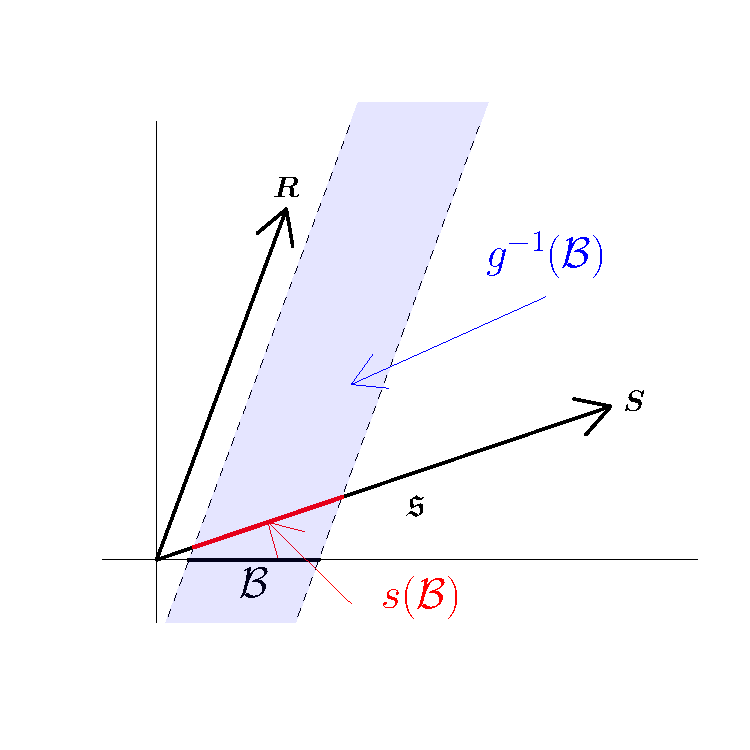
\includegraphics[width=0.6\textwidth]{Figs/probforerec_schematic.pdf}
	\caption{Summary of probabilistic forecast reconciliation. The probability that $\bm{y}_{t+h}$ lies in the red line segment under the reconciled probabilistic forecast is defined to be equal to the probability that $\bm{y}_{t+h}$ lies in the shaded blue area under the unreconciled probabilistic forecast. Note that since the smallest possible hierarchy involves three dimensions, this figure is only a schematic.}\label{fig:probfr_sch}
\end{figure}

\section{Analytical solution} \label{sec:ParamRecon}

\subsection{Density of a reconciled distribution}

In this section we describe how a reconciled distribution can be derived analytically, from an incoherent (or base) probabilistic forecast.  We restrict our attention to linear $s$ and $g$, and show that reconciliation involves changes of coordinates and marginalisation.

\begin{theo}[Reconciled density of bottom-level]\label{theo:bottomdens}
	Consider the case where reconciliation is carried out using a composition of linear mappings $s\circ g$ where $g$ combines information from all levels of the base forecast into a new density for the bottom-level.  The density of the bottom-level series under the reconciled distribution is
	\[
	\tilde{f}_{\bm{b}}(\bm{b})=|\bm{G^*}|\int \hat{f}(\bm{G}^{-}{\bm b}+\bm{G}_\perp {\bm a})d\bm{a}\,,
	\]
	where $\hat{f}$ is the density of the incoherent base probabilistic forecast, $\bm{G^-}$ is an $n\times m$ pseudo inverse of $\bm{G}$ such that $\bm{G}\bm{G}^-=\bm{I}$, $\bm{G_\perp}$ is an $n\times (n-m)$ orthogonal complement to $\bm{G}$ such that $\bm{G}\bm{G}_\perp=\bm{0}$ and $\bm{G}'_\perp\bm{G}_\perp=\bm{I}$, $\bm{G^*}=\left(\bm{G}^-\,\vdots\,\bm{G}_\perp\right)$, and $\bm{b}$ and $\bm{a}$ are obtained via the change of variables
	\[
	\bm{y}=\bm{G^*}\begin{pmatrix}\bm{b}\\\bm{a}\end{pmatrix}\,.
	\]
\end{theo}

\begin{proof}
	See Appendix \ref{Append:bottomdend&fulldens}.
\end{proof}

\begin{theo}[Reconciled density of full hierarchy]\label{theo:fulldens}
	Consider the case where a reconciled density for the bottom-level series has been obtained using Theorem~\ref{theo:bottomdens}.  The density of the full hierarchy under the reconciled distribution is
	\[
	\tilde{f}_{\bm{y}}(\bm{y})=|\bm{S^*}|\tilde{f}_{\bm b}({\bm{S^-}\bm{y}})\mathbb{1}\left\{\bm{y}\in\mathfrak{s}\right\}\,,
	\]
	where $\mathbb{1}\left\{.\right\}$ equals $1$ when the statement in braces is true and 0 otherwise and,
	\[\bm{S^*}=\begin{pmatrix}\bm{S}^-\\\bm{S}'_\perp\end{pmatrix}\,,\]
	and $\bm{S^-}$ is an $m\times n$ pseudo inverse of $\bm{S}$ such that $\bm{S}^-\bm{S}=\bm{I}$, $\bm{S_\perp}$ is an $n\times (n-m)$ orthogonal complement to $\bm{S}$ such that $\bm{S}'_\perp\bm{S}=\bm{0}$ and $\bm{S}'_\perp\bm{S}_\perp=\bm{I}$.
\end{theo}

\begin{proof}
	See Appendix \ref{Append:bottomdend&fulldens}.
\end{proof}

\subsubsection*{Example: Gaussian Distribution}

Let the incoherent base forecasts be Gaussian with mean $\hat{\bm{\mu}}$, covariance matrix $\hat{\bm{\Sigma}}$ and density,
\begin{equation}
f(\hat{\bm{y}})=(2\pi)^{-n/2}|\hat{\bm{\Sigma}}|^{-1/2}\exp\left\{-\frac{1}{2}\left[(\hat{\bm{y}}-\hat{\bm{\mu}})'\hat{\bm{\Sigma}}^{-1}(\hat{\bm{y}}-\hat{\bm{\mu}})\right]\right\}\nonumber.
\end{equation}
Using Theorem~\ref{theo:bottomdens}, the reconciled density for the bottom-level series is given by,
\begin{equation}
\tilde{f}_{\bm{b}}(\bm{b})=\int(2\pi)^{-\frac{n}{2}}\Big|\hat{\bm{\Sigma}}\Big|^{-\frac{1}{2}}|\bm{G^*}|\exp\{-\frac{1}{2}q\}d{\bm a}\nonumber\,,
\end{equation}
where $q=(\bm{G}^-{\bm{b}}+\bm{G}_{\perp}{\bm{a}}-\hat{\bm{\mu}})' \hat{\bm{\Sigma}}^{-1}(\bm{G}^-\bm{b}+\bm{G}_\perp\bm{a}-\hat{\bm{\mu}})$, can be rearranged as
\begin{align*}
	q& =
	\left(\bm{G}^*\bt-\hat{\bm{\mu}}\right)' \hat{\bm{\Sigma}}^{-1}\left(\bm{G}^*\bt-\hat{\bm{\mu}}\right)\\
	& =
	\left(\bt-\bm{G}^{*-1}\hat{\bm{\mu}}\right)' \Big[\bm{G}^{*-1}\hat{\bm{\Sigma}}\left(\bm{G}^{*-1}\right)'\Big]^{-1}
	\left(\bt-\bm{G}^{*-1}\hat{\bm{\mu}}\right)\\
    & =\left[\bt-\PQ\hat{\bm{\mu}}\right]' \left[\PQ\hat{\bm{\Sigma}}\PQ'\right]^{-1}\left[\bt-\PQ\hat{\bm{\mu}}\right],
\end{align*}
where
\[
\begin{pmatrix}
\bm{G} \\\bm{G}_{\perp}
\end{pmatrix}=\bm{G}^{*-1}.
\]

This can be recognised as a multivariate Gaussian density in $\bm{b}$ and $\bm{a}$.  The mean and covariance matrix for the margins of the first $m$ elements are $\bm{G}\hat{\bm{\mu}}$ and $\bm{G}\hat{\bm{\Sigma}}\bm{G}'$ respectively.  Marginalising out $\bm {a}$, the reconciled forecast for the bottom-level is $\tilde{\bm{b}} \sim \mathcal{N}(\bm{G}\hat{\bm{\mu}}, \bm{G}\hat{\bm{\Sigma}}\bm{G}')$.

\subsection{Elliptical distributions}

We now describe how the true predictive distribution can be recovered for elliptical distributions via linear reconciliation and a translation.  Let the base probabilistic forecast be from the elliptical class with location parameter $\hat{\bm{\mu}}$ and scale matrix $\hat{\bm{\Sigma}}$. The objective is to obtain a mean vector and covariance matrix for the reconciled distribution that are equal to those from the true DGP which we denote as $\bm{\mu}$ and $\bm{\Sigma}$ respectively.

If reconciliation is carried out by pre-multiplying by an arbitrary matrix $\bm{S}\bm{G}$ then the location and scale parameters of the reconciled distribution are $\bm{S}\bm{G}\hat{\bm{\mu}}$ and $\bm{S}\bm{G}\hat{\bm{\Sigma}}{\bm{G}}'\bm{S}'$ respectively.  If ${\bm\Omega}$ is the true scale matrix for the bottom-level series then the correct scale matrix can be recovered by setting ${\bm G}_0={\bm{\Omega}}^{1/2}\hat{\bm \Sigma}^{-1/2}$ where $\hat{\bm \Sigma}^{1/2}$ is any matrix such that $\hat{\bm \Sigma}=\hat{\bm \Sigma}^{1/2}(\hat{\bm \Sigma}^{1/2})'$, for example a Cholesky factor. To ensure conformability of matrix multiplication, ${\bm{\Omega}}^{1/2}$ must be a $m\times n$ matrix so can be set to the Cholesky factor of ${\bm{\Omega}}$ augmented with an additional $n-m$ columns of zeros.

We note that in general ${\bm S}{\bm G}_0$ is not a projection matrix.  As a consequence, even if the base forecasts are unbiased (i.e. $\hat{\bm{\mu}}=\bm{\mu}$) the reconciled forecasts will not be since ${\bm S}{\bm G}_{0}\hat{\bm{\mu}}\neq\bm{\mu}$.  To recover the correct mean, reconciliation should also include translation by ${\bm d}_{0}={\bm\mu}-{\bm S}{\bm G}_{0}\hat{\bm{\mu}}$.

Although ${\bm S}{\bm G}_0$ is not a projection matrix in general, there are some conditions under which it will be.  These are described by the following theorem.
\begin{theo}[Optimal Projection for Reconciliation]\label{theo:optrecproj}
	Let $\hat{\bm{\Sigma}}$ be the scale matrix from an elliptical but incoherent base forecast and assume base forecasts are also unbiased.  When the true predictive is also elliptical, then this can be recovered via reconciliation using a projection if $\textrm{rank}(\hat{\bm{\Sigma}}-\bm{\Sigma})\leq n-m$.
\end{theo}
\begin{proof}
	See Appendix~\ref{Appen:optrecproj}.
\end{proof}


\section{Sample based solution}\label{sec:non-para}

In practice it is often the case that samples are drawn from a probabilistic forecast since an analytical expression is either unavailable, or relies on unrealistic parametric assumptions.  A useful result is the following
\begin{theo}[Reconciled samples]
	Suppose that $\left(\hat{\bm y}^{[1]},\ldots,\hat{\bm y}^{[L]}\right)$ is a sample drawn from an incoherent density $\hat{\nu}$.  Then $\left(\tilde{\bm y}^{[1]},\ldots,\tilde{\bm y}^{[L]}\right)$ where $\tilde{\bm y}^{[l]}:=\psi(\hat{\bm y}^{[l]})$ for all $l=1,\ldots,L$ is a sample drawn from the reconciled density $\tilde{\nu}$ as defined in Definition~\ref{def:reconprob}
\end{theo}
\begin{proof}
	For any $\mathcal{A}\in\mathscr{F}_{\mathfrak{s}}$
\begin{align}
	\mbox{Pr}(\hat{{\bm y}}\in\psi^{-1}(\mathcal{A}))&=\underset{L\rightarrow\infty}{\lim}\sum\limits_{l=1}^L\mathbb{1}\left\{\hat{\bm y}^{[l]}\in\psi^{-1}(\mathcal{A})\right\}\nonumber\\
	&=\underset{L\rightarrow\infty}{\lim}\sum\limits_{l=1}^L\mathbb{1}\left\{\psi(\hat{\bm y}^{[l]})\in(\mathcal{A})\right\}\nonumber\\
	&=\mbox{Pr}(\tilde{{\bm y}}\in(\mathcal{A}))\nonumber
\end{align}
\end{proof}

This result implies that reconciling each member of a sample drawn from an incoherent distribution provides a sample from the reconciled distribution.  Such a strategy has already been used by \cite{JeoEtAl2019}, without formal justification.  We now propose a general purpose algorithm for probabilistic forecast reconciliation that overcomes a number of shortcomings of \cite{JeoEtAl2019}.

In the point forecasting setting it is common to generate forecasts from independent statistical models, allowing forecast reconciliation to be scaled up to large hierarchies.  Since a single point forecast is generated for each series there is no ambiguity as to how these should be stacked into a vector of base forecasts $\hat{\bm{y}}$.  This is no longer the case in the probabilistic setting where multiple draws are made for each series.  \cite{JeoEtAl2019} recommend some crude heuristics that can be used to form joint samples.  In Section~\ref{Subsec:Incoherent_samplePaths} we provide an alternative based on resampling forecast errors. This provides a sample from a base probabilistic forecast. A sample from the reconciled distribution can be obtained by premultiplying these draws by $\bm{S}\bm{G}$. Strategies for choosing $\bm{G}$ are discussed in Section~\ref{subsec:Optimal_recon}. \textcolor{red}{Check this cross-reference when we finish.}

\subsection{Drawing base probabilistic forecasts} \label{Subsec:Incoherent_samplePaths}
The following method only requires that one-step ahead in-sample `forecasts' $\hat{y}_{i,t}$ can be computed for each series $i$.  These are not true forecasts since they are computed over the training data $t=1,\ldots,T$; for instance  $\hat{y}_{i,t}$ may be the fitted values of $E(y_{i,t}|y_{i,t-1})$ implied by some statistical model. Let the errors $e_{i,t} = y_{i,t} - \hat{y}_{i,t}$ be stacked in a $(n \times T)$ matrix $\bm{\mathcal{E}}:=\left\{e_{i,t}\right\}_{i=1,\dots,n,t=1,\dots,T}$.  When up to $H$ step ahead forecasts are required, we randomly select $H$ consecutive columns from $\bm{\mathcal{E}}$ to form $\bm{\mathcal{E}}^b$ and repeat for $b = 1,\dots,B$.  This preserves both serial correlation of errors as well as dependence across different series.

The $\bm{\mathcal{E}}^b$ can then be used together with forecasts $\hat{\bm{y}}_{T+h}$ for $h=1,\ldots,H$ to recursively form $B$ sample paths of the full hierarchy.  As a simple example consider the case where each forecast comes from (the same) AR(1) model and $H=2$.  Then $\hat{{y}}^b_{i,T+1}=\phi{{y}}_{i,T}+e^b_{i,1}$ and $\hat{{y}}^b_{i,T+2}=\phi\hat{{y}}^b_{i,T+1}+e^b_{i,2}$ for each $i=1,\ldots,n$ and $b=1,\ldots,B$ and where $e^b_{i,h}$ is the element in row $i$ and column $h$ of $\bm{\mathcal{E}}^b$.  Each future path can be stacked into a vector $\hat{\bm{y}}^b_{T+h}:=(\hat{{y}}^b_{1,T+h},\ldots,\hat{{y}}^b_{n,T+h})'$ which in turn are stacked into a $n\times B$ matrix $\hat{\bm{\Upsilon}}_{T+h} = (\hat{\bm{y}}^1_{T+h},\dots,\hat{\bm{y}}^B_{T+h})$.

As discussed previously, reconciling each draw from an incoherent distribution yields a sample from the reconciled distribution.  Therefore setting $\tilde{\bm{\Upsilon}}_{T+h} = \bm{SG}\hat{\bm{\Upsilon}}_{T+h}$ yields a matrix whose columns $\tilde{\bm{y}}^b_{T+h} := \bm{SG}\hat{\bm{y}}^b_{T+h}$ are a sample from the reconciled distribution.  In principle $\bm{G}$ matrices from popular point forecasting reconciliation methods can be used. In Section~\ref{subsec:Optimal_recon}, we propose a way to find an optimal $\bm{G}$ for reconciling future paths by minimising a proper multivariate scoring rule.

\section{Evaluation of hierarchical probabilistic forecasts} \label{sec:evaluation}

An important issue in all forecasting problems is evaluating forecast accuracy. In the probabilistic setting, it is common to evaluate forecasts using proper scoring rules \citep[see][and references therein]{Gneiting2007,Gneiting2014}. Throughout, we follow the convention of negatively-oriented scoring rules such that smaller values of the score indicate more accurate forecasts.  In general, a scoring rule $K()$, is {\em proper} if $\E_{Q}[K(Q,\bm{\omega})] \le \E_{Q}[K(P,{\bm\omega})]$ for all $P$. When this inequality is strict for all $P\neq Q$, the scoring rule is said to be {\em strictly proper}.

Since hierarchical forecasting is by its very nature a multivariate problem (the linear constraints affect all variables), our focus is on multivariate scoring rules.  We consider the log score (LS), energy score (ES) and the variogram score (VS).  However, in our simulations we evaluate individual margins of interest using the univariate counterparts of the log score and energy score (where the latter is the CRPS).

The log score simply involves evaluating the negative log density at the value of the realisation, $LS(P,\bm\omega)=-\log f(\bm\omega)$, where $f$ is the density associated with a distribution $P$.  The log score is more commonly used when a parametric form for the density is available, however  this density can also be approximated from a sample of values drawn from the probabilistic forecast \citep[see][]{Jordan2017}.  The energy score is most commonly calculated using the following representation
\begin{equation*}\label{eq:Energy_score}
\text{ES}(P,\bm{\omega}) =
\E_{P}
||{\bm{y}}-\bm{\omega}||^\alpha -\frac{1}{2}\E_{P}||\bm{y}-\bm{y}^*||^\alpha, \,\, \alpha \in (0,2]\,,
\end{equation*}
where $\bm {y}$ and $\bm{y^*}$ are independent copies drawn from the distribution $P$.  These expectations can be easily approximated via Monte Carlo with samples drawn from the probabilistic forecast.

The energy score has been criticised by \citet{Pinson2013a} for its low discriminative ability for incorrectly specified covariances.  The variogram score  \citep{SCHEUERER2015}, overcomes this issue and is defined as
\begin{equation*}
\text{VS}({P}, \bm{\omega}) = \displaystyle\sum_{i=1}^{n}\displaystyle\sum_{j=1}^{n}w_{ij}\left(|\omega_{i} - \omega_{j}|^p - E_{P} |{y}_{i}-{y}_{j}|^p\right)^2\,,
\end{equation*}
where $y_i$ and $y_j$ are the $i^{th}$ and $j^{th}$ elements of $\bm{y}\sim P$ and $p$ is usually set to $0.5$.

In the context of probabilistic forecast reconciliation there could be two motivations for using scoring rules. The first is to compare incoherent base probabilistic forecasts to their reconciled counterparts, to see whether reconciliation improves forecast accuracy. The second is to compare two reconciled probabilistic forecasts to one another, to evaluate which choice of $\bm{G}$ performs best in practice.

\subsection{Scoring Rules for Hierarchical Time Series}

When a expression for the density of an incoherent base forecast is available, Section~\ref{sec:ProbForecasts} describes how the density of a reconciled forecast can be recovered.  With both densities can be computed, the most straightforward scoring rule to use to compare them to one another is the log score, which is simply given by the log density evaluated at the realisation.  However, the following theorem shows that the log score is improper in the setting of comparing incoherent to coherent forecasts.

\begin{theo}[Impropriety of log score]\label{theo:logS_improp}
	When the true data generating process is coherent, then the log score is improper with respect to the class of incoherent measures.
\end{theo}

\begin{proof}
	See Appendix \ref{Appen:logS_improp}.
\end{proof}

As a result of Theorem~\ref{theo:logS_improp} we recommend avoiding the log score when comparing reconciled and unreconciled probabilistic forecasts.

If a probabilistic forecast is available for any $m$ series, then a probabilistic forecast for the full hierarchy can be derived.  Definition~\ref{def:cohprob} provides an example using the bottom-level series. This suggests that it may be adequate to merely compare two coherent forecasts to one another using the bottom-level series only. We now discuss how this depends on the specific scoring rule used.

Consider a coherent probabilistic forecast with density $\tilde{f}_{\bm{y}}$ for the full hierarchy and $\tilde{f}_{\bm{b}}$ for the bottom-level series. By Theorem~\ref{theo:fulldens}, $\tilde{f}_{\bm{y}}(\bm{y})=|\bm{S}^*|\tilde{f}_{\bm{b}}(\bm{S}^-\bm{y})\mathbb{1}{\bm{y}\in\mathfrak{s}}$.  Any realisation $\bm{y}^*$ will lie on the coherent subspace and can be written as $\bm{S}\bm{b}^*$.  The expression for the log score is therefore
\begin{align}
LS(\tilde{f}_{\bm y},\bm{y}^*)&=-\log\left(|\bm{S}^*|\tilde{f}_{\bm{b}}(\bm{S}^-\bm{S}\bm{b}^*)\right)\nonumber\\
&=-\log|\bm{S}^*|-\log \tilde{f}_{\bm{b}}(\bm{b}^*).\nonumber
\end{align}
For coherent densities, the log score for the full hierarchy differs from the log score for the bottom-level series only by $-\log(|\bm{S}^*|)$. This term is independent from the choices of ${\bm G}$. As such, rankings of different reconciliation methods using the log score for the full hierarchy will not change if only the bottom-level series is used.

The same property does not hold for all scores. For example, the energy score is invariant under orthogonal transformations \citep{Szekely2013,Gneiting2007} but not true under linear transformations in general. Therefore it is possible for one method to outperform another when energy score is calculated using the full hierarchy, but for these ranking to reverse if only bottom-level series are considered.  We therefore recommend computing the energy score using the full hierarchy.  The same reasoning holds for the variogram score.  The properties of multivariate scoring rules in the context of evaluating reconciled probabilistic forecasts are summarised in Table~\ref{tab:prop}.

\begin{table}
	\caption{Properties of scoring rules for reconciled probabilistic forecasts.}
	\centering
	\begin{tabular}{lll}\hline
		Scoring Rule& Coherent v Incoherent &Coherent v Coherent\\
		\hline
		Log Score & Not proper & Ordering preserved if compared using\\ &&bottom-level only\\
		Energy/Variogram Score & Proper & Full hierarchy should be used\\
		\hline
	\end{tabular}
	
	\label{tab:prop}
\end{table}

\clearpage
\subsection{Optimal reconciliation of incoherent future paths}\label{subsec:Optimal_recon}

{\color{blue} The respective objective function can be written as,

\begin{equation} \label{eq:Obj_func_1}
\operatornamewithlimits{argmin}_{\bm{G}_h} \quad \E_{Q}[K(\tilde{\nu}_{\bm{G}_h}, \bm{y})],
\end{equation}
where $\tilde{\nu}_{\bm{G}_h}$ is the reconciled measure with respect to $\bm{G}_h$ (the subscript $h$ emphasises distinct matrices for different forecast horizons), $Q$ is the true predictive distribution, $\bm{y}\sim Q$ and $K(.,.)$ is a proper scoring rule \citep[see][and references therein]{Gneiting2007,Gneiting2014}.

To approximate the expectation in Equation~\eqref{eq:Obj_func_1} we break up the training sample into $J$ rolling windows each of length $T-J+1$.  For the $j^{th}$ rolling window we use $\bm{y}_{j},\ldots,\bm{y}_{T-J+j}$ to evaluate a $h$-step ahead base probabilistic forecast $\hat{\nu}$.  Reconciling with respect to $\bm{G}_h$ yields the distribution $\tilde{\nu}_{\bm{G}_h}$.  The expectation in Equation~\eqref{eq:Obj_func_1} can then be approximated by

\begin{equation} \label{eq:Obj_func_apprx} \E_{Q}[K(\tilde{\nu}_{\bm{G}_h}, \bm{y})]\approx\frac{1}{J}\sum_{j=1}^{J}K(\tilde{\nu}_{\bm{G}_h},\bm{y}_{T-J+j+h}).\nonumber
\end{equation}

We implement this algorithm in Section \ref{sec:Bootsrap-sim} to reconcile probabilistic forecasts in a simulation setting. Now we turn to the discussion of evaluation criteria for hierarchical probabilistic forecasts.}



\clearpage
\section{Simulations}

The aim of the simulations that follow is to evaluate the performance of both analytical and sample based reconciliation approaches for generating probabilistic hierarchical forecasts, respectively presented in Sections \ref{sec:ParamRecon} and \ref{sec:non-para}. The data generating process we consider corresponds to the 2-level hierarchical structure presented in Figure \ref{fig:twoL-hier}. Bottom-level series are first generated from ARIMA$(p,d,q)$ processes, which are in-turn aggregated to form the middle and top-level series. We consider a Gaussian and a non-Gaussian setting for the errors driving the ARIMA processes. More specifically we generate Gaussian errors jointly from a multivariate distribution, and non-Gaussian errors from a Gumbel copula model with beta margins. All details of the data generating process are presented in Appendix \ref{Append:Gauss_sim_Univ}.

For each series we generate 2002 observations from which we ignore the first 500 to avoid the impact of initial values. Using a training window of 500 observations, we fit univariate ARIMA and exponential smoothing (ETS) models to each series using the \verb|auto.arima()| and \verb|ets()| functions in the \verb|forecast| package \citep{Rforecast} in R \citep{Rcore} and generate incoherent base probabilistic forecasts assuming Gaussian errors, for $h = 1, 2$ and 3-steps ahead. \textcolor{red}{Ok this at least for the copula errors means that we have error mis-specification for the models. For example we could have used a bootstrap error rather than Gaussian. Something we may comment about below.} The incoherent base probabilistic forecasts are reconciled using the alternative approaches as described below. The process is repeated by rolling the training window forward one observation at a time. This yields 1,000 probabilistic forecasts for evaluation.

The predictive accuracy of the alternative methods is evaluated using the scoring rules presented in Section~\ref{sec:evaluation}. Results are reported in terms of skill scores, i.e., the percentage improvement of a probabilistic forecast over a reference method. A positive (negative) value indicates a percentage gain (loss) in forecast accuracy over the reference method. In order to save space in what follows we only present the results from reconciling the ARIMA incoherent base forecasts. Results and conclusions are very similar for the ETS incoherent base forecasts. These are available upon request. \textcolor{red}{Puwasala to make sure that these are available.}

\subsection{Reconciliation via the analytical solution}

We assume a Gaussian predictive density for the simulated hierarchical time series, i.e., $\hat{\bm{y}}\sim N(\hat{\bm{\mu}},\hat{\bm{\Sigma}})$. We note that the analytical tractability of the normal distribution allows for evaluation using all scoring rules (including the log-score). $\hat{\bm{\mu}}$ is given by the mean of the incoherent base probabilistic forecasts. We estimate $\hat{\bm{\Sigma}}$ from the in-sample one-step ahead forecast errors using the shrinkage estimator of \citet{Schafer2005} (as the one presented in Table \ref{table:ReconMethods}). Coherent probabilistic forecasts are then generated as $\tilde{\bm{y}}
\sim N(\bm{S}\bm{G}\hat{\bm{\mu}},\bm{S}\bm{G}\hat{\bm{\Sigma}}\bm{G}'\bm{S}')$ where ${\bm G}=(\bm{R}_{\perp}'\bm{S})^{-1}\bm{R}_{\perp}'$ and $\bm{R}'_\bot=\bm{S}'\bm{W}^{-1}$ for the different choices of $\bm{W}$ as presented in Table \ref{table:ReconMethods}.


\begin{table}[!t]
	\caption{Summary of reconciliation methods for which $\bm{S}\bm{G}$ is a projection matrix, so that ${\bm G}=(\bm{R}_{\perp}'\bm{S})^{-1}\bm{R}_{\perp}'$ and $\bm{R}'_\bot=\bm{S}'\bm{W}^{-1}$. The rows present alternative choices of $\bm{W}$. $\hat{\bm{W}}^{\text{sam}}$ is the sample variance-covariance matrix estimated from one-step ahead in-sample forecast errors from the base incoherent forecasts. $\hat{\bm{W}}^{\text{wls}}$ is a diagonal matrix with elements from $\hat{\bm{W}}^{\text{sam}}$. $\hat{\bm{W}}^{\text{shr}}$ is a shrinkage estimator proposed by \citet{Schafer2005},  where $\tau = \frac{\sum_{i \neq j}\hat{\var}(\hat{w}_{ij})}{\sum_{i \neq j}{\hat{w}}^2_{ij}}$ and  $w_{ij}$ denotes the $(i,j)$th element of $\hat{\bm{W}}^{\text{sam}}$.}\label{table:ReconMethods}
	\centering
	\begin{tabular}{l@{\hskip 0.4in}l}
		\toprule
		\textbf{Reconciliation method} & \textbf{$\bm{W}$} \\
		\midrule
		OLS             & $\bm{I}$ \\
		WLS             & $\text{diag}(\hat{\bm{W}}^{\text{sam}})$ \\
		MinT(Sample)    & $\hat{\bm{W}}^{\text{sam}}$ \\
		MinT(Shrink)    & $\tau\text{diag}(\hat{\bm{W}}^{\text{sam}}) + (1-\tau)\hat{\bm{W}}^{\text{sam}}$\\
		\bottomrule
	\end{tabular}
\end{table}






\subsubsection{Results and discussion}

Table~\ref{tab:SimResults_Gauss_MultivScores} summarises the forecasting performance of incoherent, bottom-up, OLS, WLS and two MinT reconciliation methods using log score, energy score and variogram score. The top panel refers to the Gaussian DGP whereas the bottom panel refers to the non-Gaussian DGP. Recall that the log score is improper with respect to incoherent forecasts. Therefore we calculate the skill scores with reference to the bottom-up forecasts instead of incoherent forecasts in all cases and leave blank the cell for log score of the incoherent forecasts. Further, all log scores are evaluated on the basis of bottom-level series only, however these only differ from the log scores for the full hierarchy by a fixed constant. Overall, the MinT methods provide the best performance irrespective of the scoring rule, and all methods that reconcile using information at all levels of the forecast improve upon incoherent forecasts. Bottom-up forecasts perform even worse than incoherent forecasts in some cases. These results hold for both the Gaussian as well as the non-Gaussian DGP.

Tables~\ref{tab:SimResults_Gauss_UnivScores} break down the forecasting performance of the different methods by considering univariate scores on each individual margin. We have only presented the results for forecast horizon $h=1$ and the results for rest of the forecasts horizons are presented in table \ref{Append:Gauss_sim_Univ} in Appendix.  Univariate log score and CRPS are considered, while skill scores are computed with the incoherent forecasts as a reference. When broken down in this fashion, irrespective of DGP, the methods based on MinT perform best for most series and outperform bottom-up forecasts in almost all cases.

\begin{table}[H]
	\caption{Forecast evaluation of hierarchical probabilistic forecasts for $h=1, 2$ and $3$ steps ahead. Entries show the percentage (\%) skill score with reference to the bottom-up method. A positive (negative) entry shows a gain (loss) in forecast accuracy over the reference method. The top panel shows the results from the Gaussian DGP while the bottom panel shows the results from the non-Gaussian DGP. The Log Score entries are based on the joint forecast distribution for the bottom-level, while the Energy and Variogram skill scores are based on the joint forecast distribution across the entire hierarchy.}\label{tab:SimResults_Gauss_MultivScores}
	\centering
	\resizebox{\linewidth}{!}{
		\begin{tabular}{lccccccccc}
			\toprule
			\multicolumn{1}{c}{} & \multicolumn{3}{c}{Log Score (\%)} & \multicolumn{3}{c}{Energy Score (\%)} & \multicolumn{3}{c}{Variogram Score (\%)} \\
			\cmidrule(lr){2-4} \cmidrule(lr){5-7} \cmidrule(lr){8-10}
			$h$ & 1 & 2 & 3 & 1 & 2 & 3 & 1 & 2 & 3\\
			\toprule
			\multicolumn{10}{c}{Gaussian DGP}\\
			\toprule
			Incoherent base & & & & 10.00 & 9.04 & 5.90 & -21.57 & -40.58 & -57.11\\
			Bottom-up & 0.00 & 0.00 & 0.00 & 0.00 & 0.00 & 0.00 & 0.00 & 0.00 & 0.00\\
			OLS & 0.26 & 1.20 & 1.02 & 15.00 & 15.46 & 12.43 & 0.47 & -0.35 & -1.85\\
			WLS & 1.05 & 2.70 & 3.87 & 18.00 & 18.99 & 15.92 & 1.61 & 1.69 & 1.55\\
			MinT(Sample) & 1.29 & 2.64 & 4.62 & 19.35 & 20.65 & 17.82 & 2.10 & 2.92 & 3.93\\
			MinT(Shrink) & \textbf{1.35} & \textbf{2.75} & \textbf{4.95} & \textbf{19.33} & \textbf{20.75} & \textbf{18.08} & \textbf{2.34} & \textbf{2.96} & \textbf{4.39}\\
			%		\midrule
			%		\textit{Bottom up} & $\mathbi{11.9}$ & $\mathbi{5.49}$ & $\mathbi{2.25}$ & $\mathbi{14.3}$ & $\mathbi{6.37}$ & $\mathbi{2.40}$ & $\mathbi{17.00}$ & $\mathbi{7.35}$ & $\mathbi{2.56}$\\
			\toprule
			\multicolumn{10}{c}{Non-Gaussian DGP}\\
			\toprule
			Incoherent base & & & & 8.47 & 8.94 & 9.20 & -2.79 & -2.09 & -3.62\\
			Bottom-up & 0.00 & 0.00 & 0.00 & 0.00 & 0.00 & 0.00 & 0.00 & 0.00 & 0.00\\
			OLS & 0.65 & 0.47 & 0.10 & 11.26 & 12.27 & 13.12 & 0.17 & 0.48 & -0.24\\
			WLS & 0.93 & 1.34 & 0.89 & 12.72 & 14.22 & 15.20 & 0.00 & 0.41 & -0.42\\
			MinT(Sample) & 4.40 & 4.30 & 3.42 & 15.02 & 16.94 & 17.88 & 0.59 & 1.02 & 0.64\\
			MinT(Shrink) & \textbf{4.52} & \textbf{4.55} & \textbf{4.01} & \textbf{15.04} & \textbf{16.98} & \textbf{18.00} & \textbf{0.69} & \textbf{1.34} & \textbf{0.66}\\
			
			\bottomrule
		\end{tabular}
	}
\end{table}


\begin{table}[H]
	\caption{Forecast evaluation of univariate hierarchical probabilistic forecasts for $h=1-$step ahead. Entries show the percentage (\%) skill score base on the Log-Score and CRPS with reference to the incoherent base forecasts. A positive (negative) entry shows a gain (loss) in forecast accuracy over the reference method. The left panel shows the results from the Gaussian DGP while the right panel shows the results from the non-Gaussian DGP.}\label{tab:SimResults_Gauss_UnivScores}
	\centering
	\resizebox{\linewidth}{!}{
		\begin{tabular}{lcccccccccccccc}
			\toprule
			\multicolumn{1}{c}{ } & \multicolumn{7}{c}{Gaussian} & \multicolumn{7}{c}{Non-Gaussian}\\
			\cmidrule(lr){2-8} \cmidrule(lr){9-15}
						
			Series & Tot & A & B & AA & AB & BA & BB & Tot & A & B & AA & AB & BA & BB \\
			\toprule
			\multicolumn{15}{c}{Log Score (\%)}\\
			\toprule
			Base & 0.00 & 0.00 & 0.00 & 0.00 & 0.00 & 0.00 & 0.00 & 0.00 & 0.00 & 0.00 & 0.00 & 0.00 & 0.00 & 0.00\\
			Bottom up & -23.31 & -2.46 & -1.08 & 0.00 & 0.00 & 0.00 & 0.00 & -246.37 & -1.87 & -3.11 & 0.00 & 0.00 & 0.00 & 0.00\\
			OLS & -3.92 & 3.71 & -0.42 & 1.29 & 2.39 & 0.24 & 0.12 & -84.90 & 0.08 & 2.57 & 1.07 & -0.55 & 2.25 & -0.21\\
			WLS & -0.76 & 6.19 & -0.07 & 1.77 & 3.13 & \textbf{0.33} & 0.21 & \textbf{0.35} & -0.52 & 4.07 & 1.20 & -0.74 & 3.13 & -0.26\\
			MinT(Sample) & 0.29 & \textbf{7.47} & 0.28 & 1.97 & \textbf{3.70} & 0.31 & 0.25 & -0.72 & \textbf{0.28} & \textbf{4.94} & 1.29 & -0.13 & 4.99 & \textbf{0.91}\\
			MinT(Shrink) & \textbf{0.30} & 7.44 & \textbf{0.30} & \textbf{2.00} & 3.61 &\textbf{0.33} & \textbf{0.29} & -0.26 & 0.27 & 4.91 & \textbf{1.31} & -0.11 & \textbf{5.00} & 0.87\\
			\hline
			
			\toprule
			\multicolumn{15}{c}{CRPS (\%)}\\
			\toprule
			
			Base & 0.00 & 0.00 & 0.00 & 0.00 & 0.00 & 0.00 & 0.00 & 0.00 & 0.00 & 0.00 & 0.00 & 0.00 & 0.00 & 0.00\\
			Bottom up & -103.83 & -9.87 & -3.73 & 0.16 & -0.04 & 0.10 & 0.12 & -541.40 & -4.60 & -8.99 & -0.10 & -0.12 & -0.02 & -0.08\\
			OLS & -12.61 & 12.55 & -1.69 & 4.73 & 8.21 & 0.74 & 0.83 & -96.77 & 0.55 & 6.48 & 2.70 & -1.46 & 6.19 & -0.81\\
			WLS & -2.09 & 20.26 & -0.38 & 6.35 & 10.75 & 1.07 & \textbf{1.23} & 0.01 & -1.02 & 9.95 & 2.92 & -1.90 & 8.50 & -0.96\\
			MinT(Sample) & \textbf{1.08} & \textbf{23.92} & 0.67 & 7.03 & \textbf{12.46} & 1.02 & 0.95 & -1.16 & \textbf{0.92} & \textbf{11.90} & \textbf{3.40} & -0.11 & \textbf{13.22} & \textbf{2.37}\\
			MinT(Shrink) & 0.91 & 23.74 & \textbf{0.84} & \textbf{7.13} & 12.21 & \textbf{1.18} & 1.19 & -1.16 & \textbf{0.92} & \textbf{11.90} & \textbf{3.40} & -0.11 & \textbf{13.22} & \textbf{2.37}\\
			
			\bottomrule
		\end{tabular}
	}
\end{table}

\subsection{Reconciliation via sampling}


Bootstrap approach: Generate 2102 data points for each series. Ignoring first 500 observations to avoid the impact of initial values. Choose 600 observations for outer rolling window and follow the steps in the algorithm to generate reconciled probabilistic forecasts for  h = 1, 2 and 3 steps ahead forecast horizons.  Replicate the process for 1000 times by rolling the window one step at a time. This yields 1000 forecast distributions for evaluation for all forecast horizons.


\subsection{Simulation setup for non-parametric solution}\label{sec:Bootsrap-sim}

We now implement the non-parametric approach introduced in Section \ref{sec:non-para}. Our main focus in this study is to compare different reconciliation methods to optimal reconciliation. We narrow down the study to find optimality with respect to energy score. Following equation (\ref{eq:Energy_score}) for samples from the probability distribution and for $\alpha = 1$, we can rewrite the objective function in (\ref{eq:Obj_func_apprx}) as,

\begin{equation}\label{eq:Obj_func_apprx_ES}
\operatornamewithlimits{argmin}_{\bm{G}} \frac{1}{N}\sum_{j=1}^{N}\left\{\frac{1}{B}\sum_{b=1}^{B}||\bm{SG}_h\bm{y}_{T+h,j}^b -\bm{y}_{T+h,j}||-\frac{1}{2(B-1)}\sum_{b=1}^{B-1}||\bm{SG}_h(\bm{y}_{T+h,j}^b -\bm{y}_{T+h,j}^{b+1})||\right\}
\end{equation}

First we generate $2500$ data points for each series in the hierarchy using the same DGP discussed in Section \ref{subsec:DGP}. Following the algorithm explained in Section \ref{subsec:Optimal_recon}, we choose $L=600$ observations for outer rolling window and $T=500$ observations for inner rolling window. We fit univariate ARIMA models using \verb|auto.arima()| function and generate $B=1000$ of $h=1$ to $3$ steps-ahead incoherent bootstrapped future paths following steps 2 and 3. We repeat these steps for $N=100$ times by moving the inner window one step at a time. Following step 6, we then estimate $\bm{G}_h^{Opt}$. We use numerical optimisation methods to attain the optimum. Next, we generate $\tilde{\bm{\Upsilon}}_{T+h}$ following step 7 and compute $\tilde{\bm{\Upsilon}}'_{T+h} = \bm{SG}_h\hat{\bm{\Upsilon}}'_{T+h}$ for $h=1,2,3$ as described in step 8. We use $\bm{G}_h^{Opt}$ as well as other $\bm{G}$ matrices given in Table \ref{table:ReconMethods} (in appendix) for reconciliation in step 8. Finally we repeat this whole process for $1000$ times by moving the outer rolling window one step-ahead at a time. Collect $1000$ reconciled future paths, $\tilde{\bm{\Upsilon}}_{T+h}$, from different reconciliation methods for $h=1,2,3$ and evaluate the forecasting performances.

We also note that different parameterisation methods were used for estimation $\bm{G}_h^{Opt}$. This was discussed in detail in Section \ref{Appen:ReparaG} in Appendix.

\subsubsection{Results and discussion}

We use energy score and variogram score to assess the predictive performance from different reconciliation methods. Results following from Non-Gaussian and Gaussian DGP are presented in left and right panels of Table \ref{table:Non-paraSimulation} respectively.

Mann-Whitney test was used to compare the difference of scores between reconciliation methods. The results support that the ES and VS for all reconciled forecasts are significantly lower than those of incoherent forecasts. This implies that all reconciliation methods produce coherent probabilistic forecasts with improved predictive ability compared to the incoherent forecasts. In addition to that, the MinT(Shrink) and Optimal method have similar prediction accuracy as there is no significant difference between the scores from these reconciliation methods. Although the scores are relatively larger for Gaussian than non-Gaussian data, the overall conclusions are consistent.

The simulation results from reparameterisation methods are presented in Table \ref{table:Non-paraSim_re-para} in Appendix. From these we note that the different parameterisation of $\bm{G}$ for optimal reconciliation give equivalent results irrespective to the forecast horizon or the DGP.

However we also note that optimal reconciliation required a high computational cost for larger hierarchies. Further, it requires sufficient data points to learn the $\bm{G}$ matrix. Thus we suggest using the MinT $\bm{G}$ for reconciling bootstrapped future paths for two reasons. First, it is computationally efficient relative to the optimal method, and second, it produces accurate probabilistic forecasts that are at least as good as the Optimal method with respect to the energy score.

\begin{table}
	\caption{Energy scores (ES) and variogram scores (VS) for probabilistic forecasts from different reconciliation methods are presented. Bottom row represent the scores for base forecasts which are not coherent. The smaller the scores, the better the forecasts are.} \label{table:Non-paraSimulation}
	%	\centering
	\begin{center}
		\tabcolsep=0.08cm\small
		\resizebox{\linewidth}{!}{
			\begin{tabular}{@{}lSSSSSS|SSSSSS@{}}
				\toprule
				\multicolumn{1}{c}{} & \multicolumn{6}{c|}{Energy Score} & \multicolumn{6}{c}{Variogram Score}\\
				\toprule
				 &
				\multicolumn{3}{c}{Gaussian DGP} &
				\multicolumn{3}{c|}{Non-Gaussian DGP} &
				\multicolumn{3}{c}{Gaussian DGP} &
				\multicolumn{3}{c}{Non-Gaussian DGP}\\
				\cmidrule(lr){2-4} \cmidrule(lr){5-7} \cmidrule(lr){8-10} \cmidrule(lr){11-13}
				h & {}{1} &  {2} & {3} & {1} &  {2} & {3} & {1} &  {2} & {3} & {1} &  {2} & {3}  \\
				\midrule
				Base & 11.7 & 14.6 & 17.8 & 5.71 & 5.94 & 6.27 & 5.56 & 6.61 & 7.87 & 1.28 & 1.37 & 1.49 \\
				OLS & 11.1 & 13.7 & 16.7 & 5.51 & 5.70 & 5.98 & 4.86 & 5.35 & 6.05 & 1.23 & 1.30 & 1.40 \\
				WLS & 10.7 & 13.2 & 16.0 & 5.43 & 5.60 & 5.89 & 4.86 & 5.35 & 5.86 & 1.23 & 1.30 & 1.40 \\
				MinT(Shrink)* & 10.5 & 12.8 & 15.7 & 5.33 & 5.50 & 5.77 & 4.77 & 5.24 & 5.86 & 1.19 & 1.26 & 1.34 \\
				Optimal* & 10.6 & 12.9 & 15.7 & 5.36 & 5.51 & 5.83 & 4.85 & 5.30 & 5.86 & 1.21 & 1.27 & 1.40 \\
				\bottomrule
			\end{tabular}
		}
	\end{center}
	\textit{The differences in scores between methods noted by ``*'' are statistically insignificant. The differences between these and the incoherent forecasts are statistically significant.}
\end{table}


\section{Application: Forecasting Australian domestic tourism flow}\label{sec:Application}

In this section we illustrate how the probabilistic forecast reconciliation methods can be used in practice, by forecasting domestic tourism flows in Australia. Previous studies have shown that reconciliation for this data generate more accurate point forecasts compared to the bottom-up or incoherent forecasts. For example see \citet{AthEtAl2009}, \citet{HynEtAl2011} and \citet{WicEtAl2019}. This study is the first to apply reconciliation methods for forecasting tourism in a probabilistic framework.

\subsection{Data}
As a measure of domestic tourism flows, we consider the ``overnight trips" to different destinations across the country.
%An Australian citizen going on a trip within the country, to a minimum of 40km away from the residence and spending at least one night is considered as an overnight trip.
Data are collected through the National Visitor Survey (NVS) managed by Tourism Research Australia based on an annual sample of $120,000$ Australian residents aged $15$ years or more, through telephone interviews \citep{TourismResearch2019}.

The total number of overnight trips in Australia can be naturally disaggregated through a geographic hierarchy. This hierarchy consists of 7 states \footnote{We have considered ACT as a part of New South Wales and Northern Territory as a state.} in the 1st level of disaggregation, 27 zones in the 2nd level of disaggregation and 76 regions in the bottom-level and thus comprises 110 series in total. More details about the individual series are provided in Table \ref{table:A1}.
We consider monthly overnight trips for all series spanning the period January 1998 to December 2018. This gives 152 observations per series.

\subsection{Forecasting methodology}

We apply both the parametric and non-parametric reconciliation approaches as discussed in previous sections. We use a rolling window of 100 observations as the training sample where the first training sample will span the period Jan-1998 to Apr-2006. Based on this training set we fit univariate ARIMA and ETS models for each series in the hierarchy using automated functions \verb|auto.arima()| and \verb|ets()| from the \verb|forecast| package \citep{Rforecast} in R software \citep{Rcore}.
From the estimated models we generate parametric and non-parametric probabilistic forecasts for one year ahead, i.e for $h=1,\dots,12$. For the parametric forecasts, we assume Gaussian densities and obtain the incoherent mean and variance forecasts. These are then reconciled using the methods described in Section \ref{sec:ParamRecon}. For the non-parametric forecasts, we generate the bootstrapped future paths and then reconcile each sample path as described in Section \ref{sec:non-para}. We note that we do not implement the MinT(Sample) approach as the sample size of training data set is less than the dimension of the hierarchy. Using a rolling window, one month at a time, we replicate the process until the end of the sample. This yields, $152$ 1-step ahead, $151$ 2-steps ahead through to $141$ 12-step ahead probabilistic forecasts available for evaluation. We note that we only present the results for ARIMA models in the following section. The results for ETS models are similar and we present these in the Appendix.


\subsection{Evaluation, results and discussion}

We evaluate the predictive accuracy using scoring rules. More specifically we use energy and variogram scores to assess the predictive accuracy of multivariate forecast distributions across the entire hierarchy as well as for the different disaggregation levels. CRPS is used to assess the predictive accuracy of univariate forecast distributions for each series in the hierarchy. We calculate average scores over the replications for each forecast horizon separately. In the results that follow we present skill scores for each of the coherent predictive distributions with reference to the incoherent distributions. A positive (negative) values in the skill score indicates a gain (loss) in forecast accuracy over the incoherent forecast distribution.

\begin{figure}
	\centering
	\small
	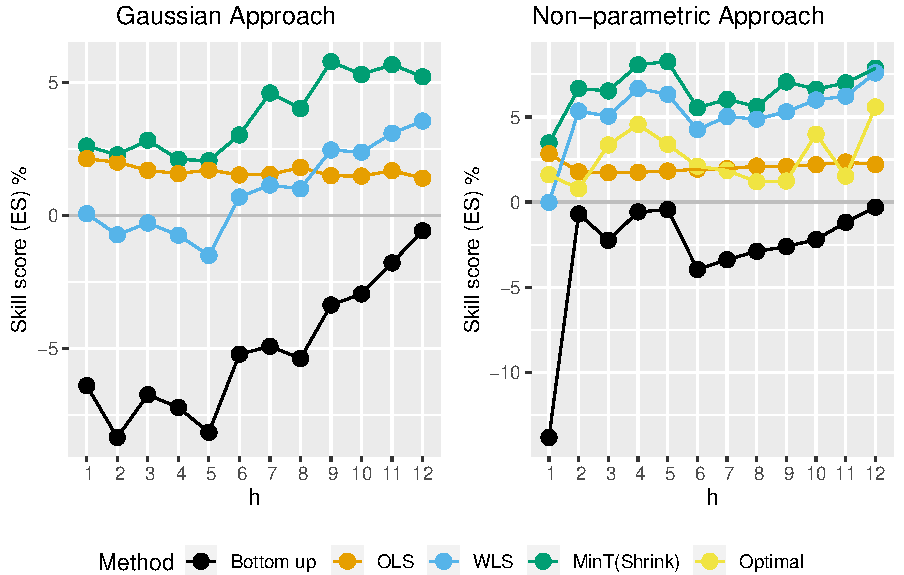
\includegraphics[width= .95\textwidth]{Empirical-results/Results-ARIMA/Overall_Summary.pdf}
	\caption{Skill scores based on energy score with reference to incoherent forecasts for multivariate predictive distribution across the entire hierarchy from different methods. A positive (negative) skill score indicates a gain (loss) in forecast accuracy over the incoherent forecast distribution. The left panel shows the results from the Gaussian approach where the right panel shows the results from the non-parametric approach.}\label{fig:EmpResults_AllTS}
\end{figure}

\begin{figure}
	\centering
	\small
	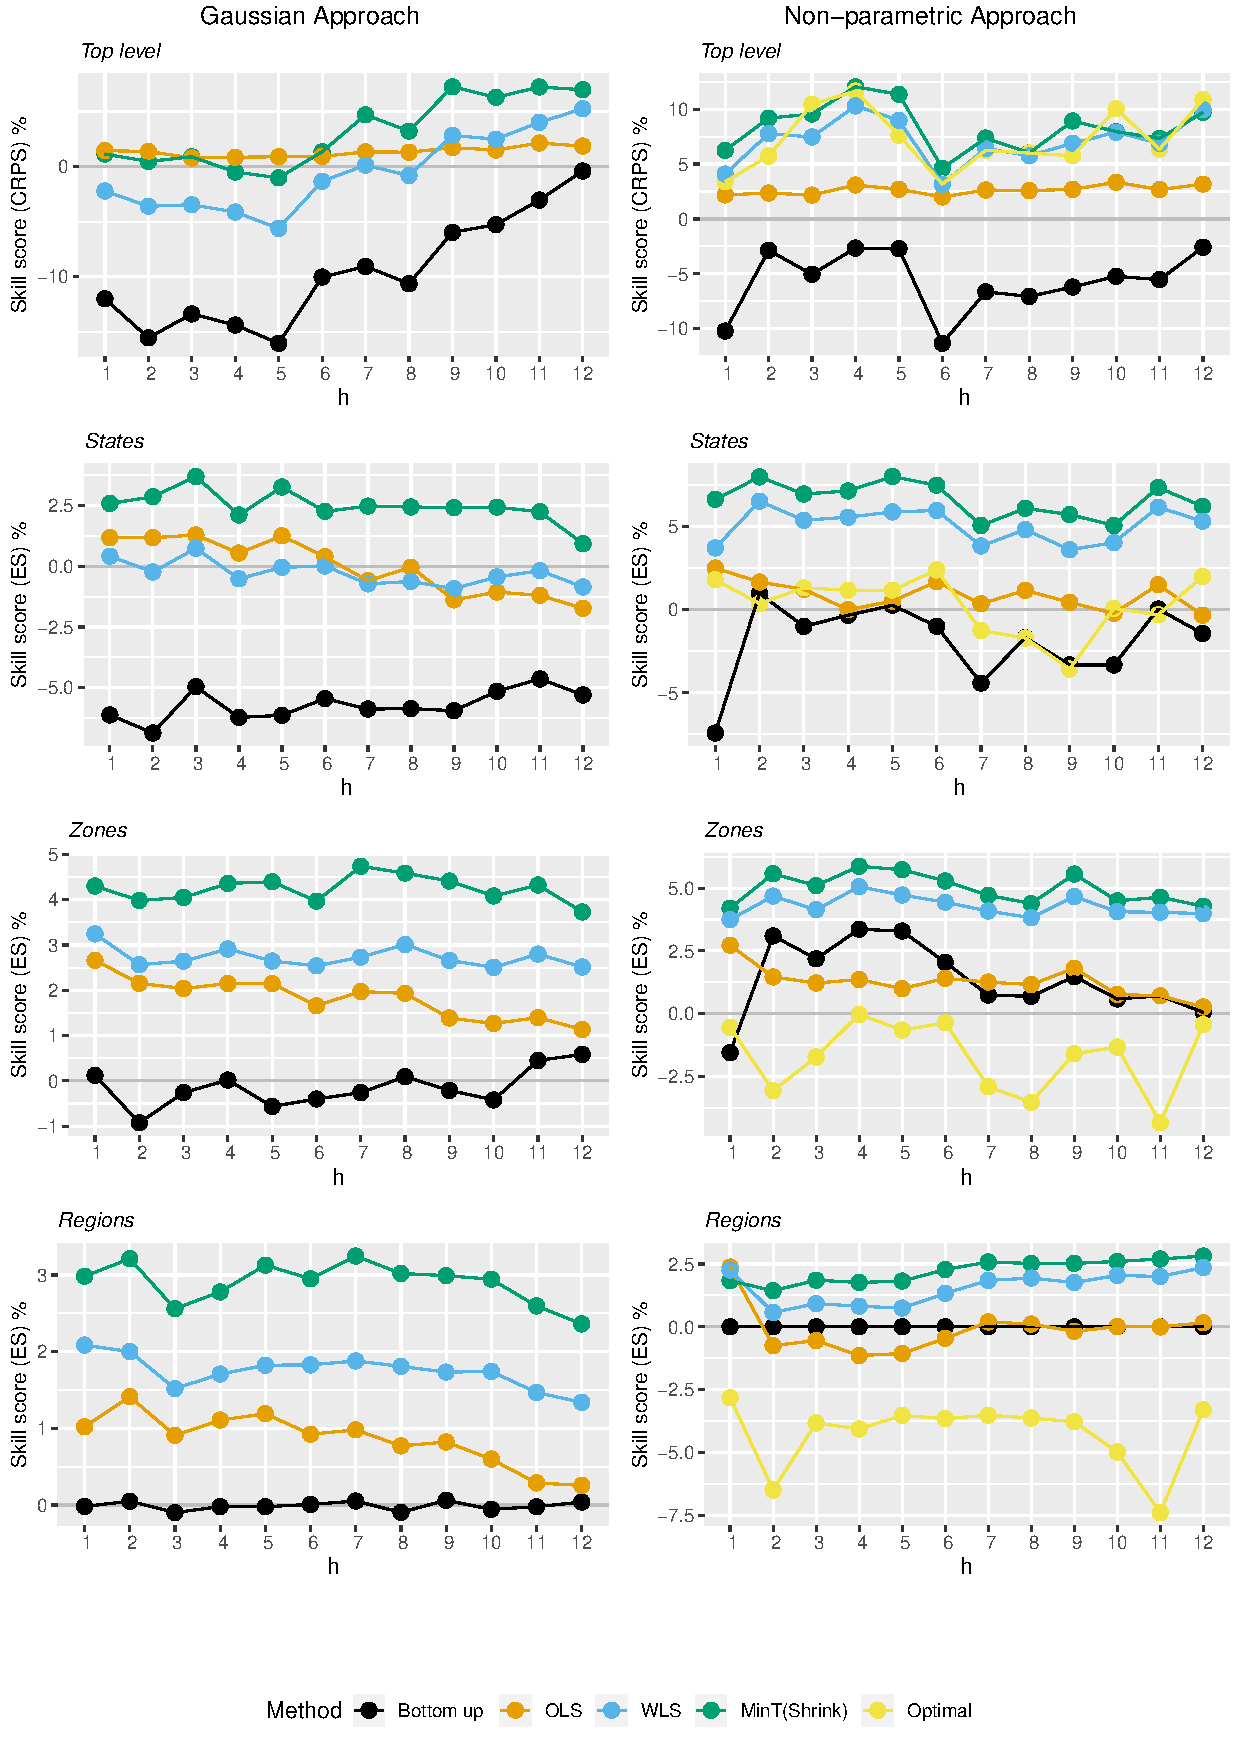
\includegraphics[width= 0.8\textwidth, height= 0.85\textheight]{Empirical-results/Results-ARIMA/Levels_Summary.pdf}
	\caption{Skill scores for multivariate probabilistic forecasts across different levels of the hierarchy. A positive (negative) skill score indicates a gain (loss) in forecast accuracy over the incoherent forecast distribution. Results from the Gaussian approach are presented in the left panel while results from the non-parametric approach are presented in the right panel.}\label{fig:EmpResults_Levels}
\end{figure}

%\begin{figure}
%	\centering
%	\small
%	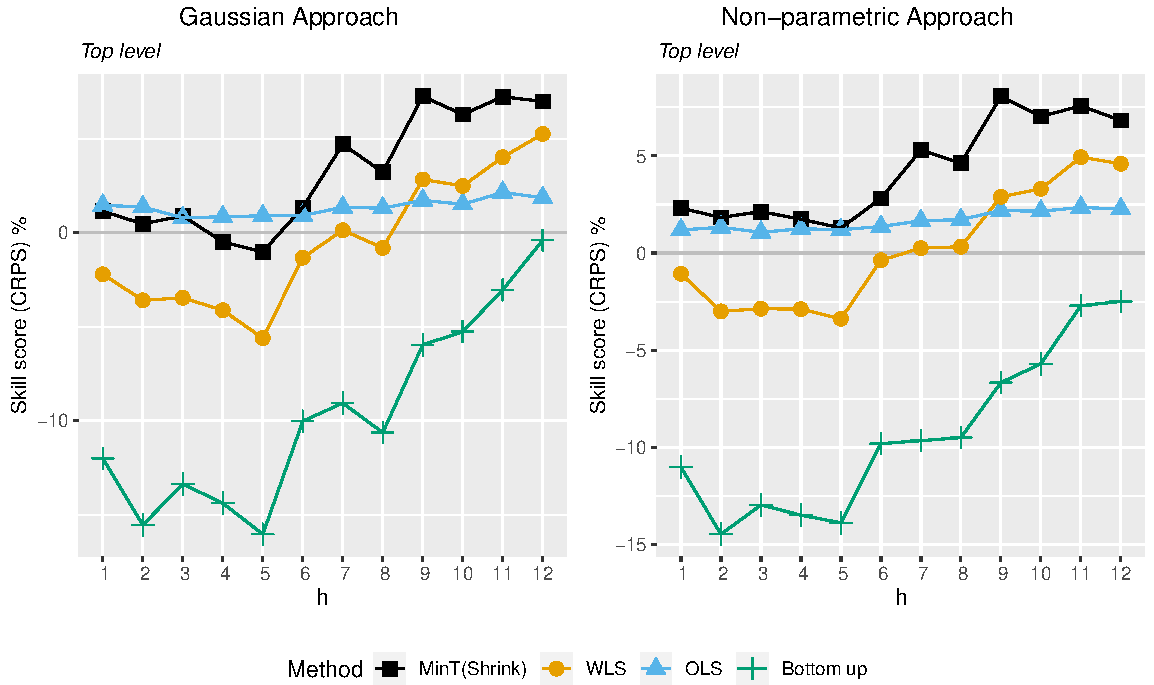
\includegraphics[width= \textwidth]{Empirical-results/UniVScore_TopLevel_ARIMA.pdf}
%	\caption{Skill score based on CRPS (with reference to the incoherent forecasts) for univariate probabilistic forecasts for the Total (top level) overnight trips. A positive (negative) skill score indicates a gain (loss) in forecast accuracy over the incoherent forecast distribution. Left panel shows the results from the Gaussian approach and right panel shows the results from the non-parametric approach. }\label{fig:EmpResults_TopLevel}
%\end{figure}

Figure \ref{fig:EmpResults_AllTS} shows the skill scores with respect to the multivariate predictive distributions across the entire hierarchy from the different methods. Figure \ref{fig:EmpResults_Levels} shows the evaluation across each level. The top panels present the results from the Gaussian approach while the bottom panels present the results from the non-parametric approach. Both figures show that almost all reconciliation methods improve forecast accuracy irrespective of whether the parametric or non-parametric approaches are implemented. Furthermore, the bottom-up approach shows losses compared to the incoherent forecasts at all forecast horizons. This reflects the fact that bottom-level series are noisier and therefore more challenging to forecast. Finally and most importantly, MinT(Shrink) outperforms all probabilistic forecast reconciliation methods for both parametric and non-parametric approaches.

Figure \ref{fig:EmpResults_TopLevel} shows the predictive accuracy of the univariate forecast distributions for the Total overnight trips. OLS and MinT(Shrink) reconciliation methods show gains in accuracy for the top level of the hierarchy for both Gaussian and non-parametric approaches.





\section{Conclusions}\label{sec:conclusions_chap3}

Although hierarchical point forecasting is well studied in the literature, there has been a relative lack of attention given to the probabilistic setting. We fill this gap in the literature by providing a mathematically rigorous formulation of coherence and reconciliation for probabilistic forecasts.

The geometric interpretation of point forecast reconciliation can be extended to the probabilistic setting. We have also discussed strategies for evaluating probabilistic forecasts for hierarchical time series advocating the use of multivariate scoring rules on the full hierarchy, while establishing a key result that the log score is not proper with respect to incoherent forecasts.

We have shown that for elliptical distributions the true predictive density can be recovered by linear reconciliation and we have established conditions for when this is a projection. Although this projection cannot feasibly be obtained in practice, a projection similar to the MinT approach provides a good approximation in applications. This is supported by the results of a simulation study as well as the empirical application.

We have further proposed a novel non-parametric approach for obtaining coherent probabilistic forecasts for when the parametric densities are unavailable. Initially this method involves generating thousands of sample paths using bootstrapped forecast errors. Then each sample path is reconciled via projections. Using an extensive simulation setting we have shown that the MinT projection is at least as good as the optimal projection with respect to minimising Energy score. Further we have shown in an empirical application that reconciled probabilistic forecasts via MinT show gains in the forecast accuracy over incoherent and bottom-up forecasts.


In many ways this chapter sets up a substantial future research agenda. For example, having defined what amounts to an entire class of reconciliation methods for probabilistic forecasts it will be worthwhile investigating which specific projections are optimal. This is likely to depend on the specific scoring rule employed as well as the properties of the base forecasts. Another avenue worth investigating is to consider whether it is possible to recover the true predictive distribution for non-elliptical distributions via a non-linear function $g(.)$.

\newpage

\appendix

\section{Proof of Theorem~\ref{theo:bottomdens} and Theorem~\ref{theo:fulldens}} \label{Append:bottomdend&fulldens}

Consider the region $\mathcal{I}$ given by the Cartesian product of intervals $(l_1,u_1),(l_2,u_2),\ldots(l_m,u_m)$.  We derive the probability that the bottom-level series lie in $\mathcal{I}$, i.e. $\mbox{Pr}(\bm{l}\succ\bm{b}\succ\bm{u})$, where ${\bm l}=(l_1,l_2,\ldots,l_m)$, ${\bm u}=(u_1,u_2,\ldots,u_m)$ and $\succ$ denotes element-wise inequality between vectors.  The pre-image of $\mathcal{I}$ under $g$ can similarly be denoted as all points ${\bm y}$ satisfying $\bm{l}\succ\bm{G}\bm{y}\succ\bm{u}$.  Using Definition~\ref{def:reconprob},
\[
\mbox{Pr}(\bm{l}\succ\bm{b}\succ\bm{u})=\int\limits_{\bm{l}\succ\bm{G}\bm{y}\succ\bm{u}}\hat{f}(\bm{y})d{\bm y}\,,
\]
where $\hat{f}$ is the density of the base probabilistic forecast.  Now consider a change of variables to an $n$-dimensional vector ${\bm z}$ where $\bm{y}={\bm G^*}{\bm z}$. Recall, ${\bm G^*}=\left({\bm G^{-}}\,\vdots\,{\bm G_\perp}\right)$, ${\bm G^{-}}$ is a pseudo inverse of $\bm{G}$ and ${\bm G_\perp}$ is an orthogonal complement of $\bm{G}$.  By the change of variables

\begin{align}
\mbox{Pr}(\bm{l}\succ\bm{b}\succ\bm{u})&=\int\limits_{\bm{l}\succ\bm{G}\bm{y}\succ\bm{u}}\hat{f}(\bm{y})d{\bm y}\nonumber\\
&=\int\limits_{\bm{l}\succ\bm{G}\bm{G}^*\bm{z}\succ\bm{u}}\hat{f}(\bm{G}^*\bm{z})|\bm{G}^*|d{\bm z}\nonumber\\
&=\int\limits_{\bm{l}\succ\bm{z}_1\succ\bm{u}}\hat{f}(\bm{G}^*\bm{z})|\bm{G}^*|d{\bm z}\nonumber\,,
\end{align}
where $\bm{z}_1$ denotes the first $m$ elements of $\bm z$.  Letting $\bm{a}$ denote the last $n-m$ elements of $\bm{z}$ the integral above can be written as
\[
\mbox{Pr}({\bm b}\in \mathcal{I})=\int\limits_{\bm{l}\succ\bm{z}_1\succ\bm{u}}\int\hat{f}(\bm{G}^{-}\bm{z}_1+\bm{G}_{\perp}\bm{a})|\bm{G}^*|d{\bm a}d{\bm z}_1\nonumber\\
\]
Replacing ${\bm z}_1$ with ${\bm b}$, it can be seen that the term inside the outer integral is a density for the bottom-level series. Therefore

\begin{equation}
\tilde{f}_{\bm{b}}(\bm{b})=\int\hat{f}(\bm{G}^{-}\bm{b}+\bm{G}_{\perp}\bm{a})|\bm{G}^*|d{\bm a}\,,
\label{eq:densb}
\end{equation}
is the density of ${\bm b}$. To obtain the density of the full hierarchy we first augment the density in Equation \eqref{eq:densb} by $n-m$ variables denoted $\bm{u}$

\begin{equation}
f(\bm{b},\bm{u})=\tilde{f}_b(\bm{b})\mathbb{1}\left\{\bm{u}=0\right\}\,,
\end{equation}
such that the density $f(\bm{b},\bm{u})$ is a density for $n$-dimensional vector that is degenerate across the dimensions corresponding to $\bm{u}$.  Using the change of variables,
\[
\bm{y}=\left(\bm{S}\,\vdots\,\bm{S}_{\perp}\right)\begin{pmatrix}\bm{b}\\\bm{u}
\end{pmatrix}\,.
\]
and noting the inverse of $\left(\bm{S}\,\vdots\,\bm{S}_{\perp}\right)$ is given by
\[
\bm{S}^*:=\begin{pmatrix}\bm{S}^{-}\\\bm{S}'_{\perp}\end{pmatrix}\,,
\]
it can be seen that $\bm{b}=\bm{S}^-\bm{y}$ and $\bm{u}=\bm{S}'_\perp\bm{y}$.  Applying this change of variables yields the density
\[
\tilde{f}_{\bm{y}}(\bm{y})=|\bm{S}^*|\tilde{f}_{\bm b}(\bm{S}^-\bm{y})\mathbb{1}\left\{\bm{S}'_\perp\bm{y}=\bm{0}\right\}\,.
\]
Since $\bm{S}'_\perp$ is the orthogonal complement of $\bm{S}$ and since the columns of $\bm{S}$ span the coherent subspace, the statement $\bm{S}'_\perp\bm{y}=0$ is equivalent to the statement $\bm{y}\in\mathfrak{s}$.  As such, the reconciled density is given by
\[
\tilde{f}_{\bm{y}}(\bm{y})=|\bm{S}^*|\tilde{f}_b(\bm{S}^-\bm{y})\mathbb{1}\left\{\bm{y}\in\mathfrak{s}\right\}.
\]
\section{Proof of Theorem~\ref{theo:optrecproj}}
\label{Appen:optrecproj}

To illustrate let
\[
\hat{\bm{\Sigma}}=\bm{\Sigma}+{\bm D}=\bm{S}\bm{\Omega}{\bm{S}}'+{\bm D}\,.
\]
If reconciliation is carried out via a projection onto $\mathfrak{s}$, then $\bm{S}\bm{G}\bm{S}=\bm{S}$ and
\begin{align}
\tilde{\bm{\Sigma}}&=\bm{S}\bm{G}\hat{\bm{\Sigma}}\bm{G}'\bm{S}'\nonumber\\
&\bm{S}\bm{G}\bm{S}\bm{\Omega}\bm{S}'\bm{G}'{\bm{S}}'+\bm{S}\bm{G}{\bm D}\bm{G}'\bm{S}'\nonumber\\
&\bm{S}\bm{\Omega}{\bm{S}}'+\bm{S}\bm{G}{\bm D}\bm{G}'\bm{S}'\nonumber\\
&\bm{\Sigma}+\bm{S}\bm{G}{\bm D}\bm{G}'\bm{S}'\nonumber\,.
\end{align}
Therefore to recover the true predictive using a projection, some ${\bm G}_0$ must be found such that ${\bm G}_0{\bm D}=\bm{0}$. Let the eigenvalue decomposition of $\bm {D}$ be given by  ${\bm R}{\bm \Lambda}{\bm R}'$ , where ${\bm R}$ is an $n\times q$ matrix with $q=\textrm{rank}({\bm{D}})$ and ${\bm\Lambda}$ is an $q\times q$ diagonal matrix containing non-zero eigenvalues of ${\bm D}$.  By the rank nullity theorem, $\bm{R}$ will have an orthogonal complement $\bm{R}_{\perp}$ of dimension $n\times (n-q)$.  If $q=n-m$ then the number of columns of $\bm{R}_{\perp}$ is $m$ and ${\bm G}_0$ can be formed as the $m\times n$ matrix $(\bm{R}_{\perp}'\bm{S})^{-1}\bm{R}_{\perp}'$.  If $q<n-m$ the number of columns of $\bm{R}_{\perp}$ is greater than $m$, and any $m$ columns of $\bm{R}_{\perp}$ can be used to form ${\bm G}_0$ in a similar fashion.  However when $q>n-m$, $\bm{R}_{\perp}$ is less than $m$ and no such $m\times n$ matrix ${\bm G}_0$ can be formed.  Therefore the true predictive can only be recovered via a projection when $\textrm{rank}({\bm D})\leq n-m$.

With respect to the location, if $\bm{SG}$ is a projection then reconciled forecasts will be unbiased as long as the base forecasts are also unbiased.  When base forecasts are biased they can be bias corrected before reconciliation as described by \cite{PanEtAl2019HF} in the point forecasting setting.

\section{Proof of Theorem~\ref{theo:logS_improp}}\label{Appen:logS_improp}

The proof relies on the following change of variables,
\[
\bm{y}=\left(\bm{S}\,\vdots\,\bm{S_\perp}\right)\begin{pmatrix}\bm{b}\\\bm{u}\end{pmatrix}.
\]
Also recall from the proof of Theorem~\ref{theo:fulldens} that $\bm{S}^*=\left(\bm{S}\,\vdots\,\bm{S_\perp}\right)^{-1}$

Let the density of the true predictive $f(\bm{y})$ after a change of variables, be given by $|\bm{S^*}|^{-1}f_{\bm b}(\bm{b})\mathbb{1}\left\{\bm{u}=\bm{0}\right\}$.  To prove that the log score is improper we construct an incoherent base density $\hat{f}$ such that $E_f\left[LS\left(\hat{f},\bm{y}\right)\right]<E_f\left[LS\left(f,\bm{y}\right)\right]$. This incoherent density is constructed, so that after the same change of variables it can be written as $|\bm{S^*}|^{-1}\hat{f}_{\bm b}(\bm{b})\hat{f}_{\bm{u}}(\bm{u})$. We require $\hat{f}_{\bm u}(\bm{0})>1$, i.e., ${\bm u}$ is highly concentrated around $\bm{0}$ but still non-degenerate. An example is an independent normal with mean 0 and variances less than $(2\pi)^{-1}$. Now, let $\bm{y}^*$ be a realisation from $f$. Premultiply $\bm{y}^*$ by $\bm{S}^*$ and let the first $m$ elements be $\bm{b^*}$.  For the remaining elements ${\bm u}^*={\bm 0}$, since $\bm{y}^*\in\mathfrak{s}$.  The log score for $f$ is thus,	
\begin{align}
LS\left(f,\bm{y}^*\right) &= -\log f(\bm{y}^*) \nonumber\\
&=-\log|\bm{S^*}|-\log f_{\bm{b}}\left(\bm{b}^*\right)-\log\left(\mathbb{1}\left\{\bm{u}^*=\bm{0}\right\}\right)\label{eq:diraccancel}\\
&=-\log|\bm{S^*}|-\log f_{\bm{b}}\left(\bm{b}^*\right),\nonumber
\end{align}
where the third term in Equation~\ref{eq:diraccancel} is equal to zero since $\bm{u}^*=\bm{0}$.  The log score for $\hat{f}$ is
\[
LS\left(\hat{f},\bm{y}^*\right) = -\log|\bm{S^*}|-\log f_{\bm{b}}(\bm{b}^*)- \log f_{\bm u}(\bm{0})\,.
\]
Since $f_{\bm u}(\bm{0})>1$ by construction, $-\log f_{\bm u}(\bm{0})<0$, therefore
\[
LS\left(\hat{f},\bm{y}^*\right) <-\log|\bm{S^*}|-\log f_{\bm b}(\bm{b}^*)=LS\left(f,\bm{y}^*\right)
\]
Since this holds for any possible realisation, it will also hold after taking expectations (by the monotonicity of expectations).  Thus $\hat{f}$ violates the condition for a proper scoring rule.

\section{Data generating process}

The hierarchy considered in the simulations is the 2-level structure shown in Figure \ref{fig:twoL-hier}. Data are first generated for the bottom-level series from
\begin{align*}
y_{AA,t} &= w_{AA,t} + u_t - 0.5v_t,\\
y_{AB,t} &= w_{AB,t} - u_t - 0.5v_t,\\
y_{BA,t} &= w_{BA,t} + u_t + 0.5v_t,\\
y_{BB,t} &= w_{BB,t} - u_t + 0.5v_t,
\end{align*}
where $w_{AA,t},w_{AB,t},w_{BA,t},w_{BB,t}$ are ARIMA$(p,d,q)$ processes with error terms \linebreak $\varepsilon_{AA,t},\varepsilon_{AB,t},\varepsilon_{BA,t},\varepsilon_{BB,t}$. $(p,q)$ and $(d)$ take integer values from $\{1,2\}$ and $\{0,1\}$ respectively with equal probability and the parameters for the AR and MA components are randomly and uniformly selected from $[0.3,0.5]$ and $[0.3,0.7]$ respectively. $u_t \sim \mathcal{N}(0,\sigma^2_u)$ and $v_t \sim \mathcal{N}(0,\sigma^2_v)$. Aggregating the bottom-level series gives the series for the aggregated levels. More specifically,
\begin{align*}
y_{A,t} &= w_{AA,t} + w_{AB,t} - v_t,\\
y_{B,t} &= w_{BA,t} + w_{BB,t} + v_t,\\
y_{Tot,t} &= w_{AA,t} + w_{AB,t} + w_{BA,t} + w_{BB,t}.
\end{align*}


\subsubsection*{Gaussian errors}

The errors driving the bottom-level ARIMA processes are jointly generated from a Normal distribution. More specifically, $\{\varepsilon_{AA,t},\varepsilon_{AB,t},\varepsilon_{BA,t},\varepsilon_{BB,t}\} \overset{iid}{\sim} \mathcal{N}(\bm{0}, \bm{\Sigma})~\forall t$. A commonly observed feature of hierarchical time series in practice, is that upper-level aggregated series are relatively less noisy than their corresponding lower-level components. This is due to the smoothing effect of aggregation, eliminating some random variation. Similarly to \cite{WicEtAl2019}, setting
\begin{equation*}\label{eq:SigmaGaussian}
\bm{\Sigma} =
\begin{pmatrix}
5.0 & 3.1 & 0.6 & 0.4 \\
3.1 & 4.0 & 0.9 & 1.4 \\
0.6 & 0.9 & 2.0 & 1.8 \\
0.4 & 1.4 & 1.8 & 3.0 \\
\end{pmatrix}
\end{equation*} and $\sigma^2_u=28$ and $\sigma^2_v=22$ ensures that the following inequalities are satisfied. 


\begin{align*}
\var(\varepsilon_{AA,t} + \varepsilon_{AB,t} + \varepsilon_{BA,t} + \varepsilon_{BB,t})
\le \var(\varepsilon_{AA,t}+\varepsilon_{AB,t}-v_t)
\le \var(\varepsilon_{AA,t}+u_t-0.5v_t),\\
\var(\varepsilon_{AA,t} + \varepsilon_{AB,t} + \varepsilon_{BA,t} + \varepsilon_{BB,t})
\le \var(\varepsilon_{AA,t}+\varepsilon_{AB,t}-v_t)
\le \var(\varepsilon_{AB,t}-u_t-0.5v_t),\\
\var(\varepsilon_{AA,t} + \varepsilon_{AB,t} + \varepsilon_{BA,t} + \varepsilon_{BB,t})
\le \var(\varepsilon_{BA,t}+\varepsilon_{BB,t}+v_t)
\le \var(\varepsilon_{BA,t}+u_t+0.5v_t),\\
\var(\varepsilon_{AA,t} + \varepsilon_{AB,t} + \varepsilon_{BA,t} + \varepsilon_{BB,t})
\le \var(\varepsilon_{BA,t}+\varepsilon_{BB,t}+v_t)
\le \var(\varepsilon_{BB,t}-u_t+0.5v_t).\\
\end{align*}


\subsubsection*{Non-Gaussian errors}

Non-Gaussian errors are generated from a Gumbel copula with beta margins. Using a copula model helps impose a non-linear dependence structure among the series. A two dimensional Gumbel copula is given by,
\begin{equation*}
C_\theta(e_1, e_2) = exp\{-[(-ln(e_1))^\theta + (-ln(e_2))^\theta]^{1/\theta}\}.
\end{equation*}
We generate random variates $\{e_{AA}, e_{AB}\}$ from $C_{\theta=10}(.)$ and $\{e_{BA}, e_{BB}\}$ from $C_{\theta=8}(.)$ for series $\{AA, AB\}$ and $\{BA, BB\}$ respectively. We generate the ARIMA errors, $\{\varepsilon_{AA}, \varepsilon_{AB}, \varepsilon_{BA}, \varepsilon_{BB}\}$ as the quantiles from beta distributions with shape parameters $\alpha = 1$ and $\beta = 3$ that correspond to $\{e_{AA}, e_{AB}, e_{BA}, e_{BB}\}$.
We then choose $\sigma^2_u = 10$ and $\sigma^2_v = 7$ such that they satisfy the inequalities explained before. 


 \textcolor{red}{Tas to double check.}


\subsection{Simulation results from parametric solution for marginal forecast distributions}\label{Append:Gauss_sim_Univ}

\begin{table}[H]
	\caption{Comparison of incoherent vs coherent forecasts based on the univariate forecast distribution of each series. Each entry represents the percentage skill score with reference to the incoherent forecasts based on ``CRPS" and ``LS". These entries show the percentage increase in score for different forecasting methods relative to the incoherent forecasts for $h=2$ step-ahead forecast. Results from the Gaussian DGP are presented in the top panel whereas the results from the non-Gaussian DGP are presented in the bottom panel}\label{tab:SimResults_Gauss_UnivScores_h2}
	\centering
	\resizebox{\linewidth}{!}{
		\begin{tabular}{lcccccccccccccc}
			\toprule
			\multicolumn{1}{c}{ } & \multicolumn{7}{c}{Gaussian} & \multicolumn{7}{c}{Non-Gaussian}\\
			\cmidrule(lr){2-8} \cmidrule(lr){9-15}
			Series & Tot & A & B & AA & AB & BA & BB & Tot & A & B & AA & AB & BA & BB \\
			\toprule
			\multicolumn{15}{c}{Log Score (\%)}\\
			\toprule
			Base & 0.00 & 0.00 & 0.00 & 0.00 & 0.00 & 0.00 & 0.00 & 0.00 & 0.00 & 0.00 & 0.00 & 0.00 & 0.00 & 0.00\\
			Bottom up & 1.06 & -2.32 & -0.52 & -0.01 & -0.02 & 0.00 & 0.00 & -68.47 & -1.67 & -2.84 & 0.00 & 0.00 & -0.01 & 0.00\\	
			OLS & \textbf{1.34} & 2.94 & -2.07 & 1.85 & 3.76 & -0.79 & 0.02 & -14.27 & -0.12 & 3.44 & 1.15 & -0.73 & 2.74 & -0.32\\
			WLS & 0.21 & 5.14 & -1.09 & \textbf{2.23} & 5.35 & -0.45 & 0.22 & -0.15 & -1.09 & 5.55 & 1.24 & -1.00 & 3.96 & -0.38\\	
			MinT(Sample) & -0.47 & \textbf{6.48} & 0.12 & 1.97 & 6.61 & -0.10 & 0.25 & -1.53 & \textbf{0.31} & \textbf{6.87} & 1.25 & -0.24 & 6.01 & 0.76\\
			MinT(Shrink) & -0.35 & 6.41 & \textbf{0.14} & 2.08 & \textbf{6.72} & -0.09 & \textbf{0.33} & -1.16 & 0.29 & 6.83 & \textbf{1.30} & -0.18 & \textbf{6.12} & \textbf{0.80}\\		
			\toprule
			\multicolumn{15}{c}{CRPS (\%)}\\
			\toprule
			Base & 0.00 & 0.00 & 0.00 & 0.00 & 0.00 & 0.00 & 0.00 & 0.00 & 0.00 & 0.00 & 0.00 & 0.00 & 0.00 & 0.00\\
			Bottom up & -53.21 & -9.30 & -1.99 & -0.17 & 0.07 & -0.16 & 0.01 & -273.80 & -4.20 & -8.78 & -0.17 & 0.09 & 0.03 & -0.10\\
			OLS & -4.84 & 12.67 & -6.63 & 6.24 & 11.75 & -2.88 & 0.35 & -44.06 & -0.18 & 8.72 & 2.95 & -1.85 & 7.61 & -1.19\\
			WLS & -0.25 & 20.18 & -3.29 & 7.60 & 15.98 & -1.86 & 1.06 & -0.11 & -2.50 & 13.87 & 3.34 & -2.51 & 10.79 & -1.27\\
			MinT(Sample) & 0.64 & \textbf{23.47} & 0.47 & 7.34 & 19.21 & -0.41 & 0.82 & -0.70 & \textbf{0.71} & \textbf{16.53} & \textbf{3.67} & -0.11 & \textbf{16.19} & \textbf{2.29}\\
			MinT(Shrink) & \textbf{0.76} & 23.45 & \textbf{0.52} & \textbf{7.47} & \textbf{19.36} & -0.59 & \textbf{1.08} & -0.70 & \textbf{0.71} & \textbf{16.53} & \textbf{3.67} & -0.11 & \textbf{16.19} & \textbf{2.29}\\
			\bottomrule
		\end{tabular}
	}
\end{table}

\begin{table}[H]
	\caption{Comparison of incoherent vs coherent forecasts based on the univariate forecast distribution of each series. Each entry represents the percentage skill score with reference to the incoherent forecasts based on ``CRPS" and ``LS". These entries show the percentage increase in score for different forecasting methods relative to the incoherent forecasts for $h=3$ step-ahead forecast. Results from the Gaussian DGP are presented in the top panel whereas the results from the non-Gaussian DGP are presented in the bottom panel}\label{tab:SimResults_Gauss_UnivScores_h3}
	\centering
	\resizebox{\linewidth}{!}{
		\begin{tabular}{lcccccccccccccc}
			\toprule
			\multicolumn{1}{c}{ } & \multicolumn{7}{c}{Gaussian} & \multicolumn{7}{c}{Non-Gaussian}\\
			\cmidrule(lr){2-8} \cmidrule(lr){9-15}
			Series & Tot & A & B & AA & AB & BA & BB & Tot & A & B & AA & AB & BA & BB \\
			\toprule
			\multicolumn{15}{c}{Log Score (\%)}\\
			\toprule
			Base & 0.00 & 0.00 & 0.00 & 0.00 & 0.00 & 0.00 & 0.00 & 0.00 & 0.00 & 0.00 & 	0.00 & 0.00 & 0.00 & 0.00\\
			Bottom up & \textbf{27.18} & -0.30 & 0.10 & -0.03 & -0.04 & 0.00 & 0.00 & 10.59 & -1.77 & -2.27 & 0.00 & 0.00 & -0.01 & 0.00\\
			OLS & 7.73 & 0.45 & -6.60 & 1.99 & 4.43 & -2.22 & -1.28 & 19.51 & -0.32 & 4.27 & 1.18 & -0.76 & 3.25 & -0.35\\
			WLS & 1.58 & 0.95 & -4.36 & \textbf{2.43} & 6.58 & -1.47 & -0.76 & -0.40 & -1.60 & 6.78 & \textbf{1.23} & -1.12 & 4.78 & -0.41\\
			MinT(Sample) & -1.44 & \textbf{1.97} & -1.10 & 2.03 & 8.56 & -0.53 & -0.26 & -1.61 & \textbf{0.31} & \textbf{8.35} & 1.16 & -0.58 & 6.71 & 0.64\\
			MinT(Shrink) & -0.99 & 1.82 & -0.91 & 2.25 & \textbf{8.82} & -0.54 & -0.08 & -1.35 & 0.25 & 8.28 & 1.22 & -0.47 & \textbf{6.92} & \textbf{0.76}\\
			\toprule
			\multicolumn{15}{c}{CRPS (\%)}\\
			\toprule
			Base & 0.00 & 0.00 & 0.00 & 0.00 & 0.00 & 0.00 & 0.00 & 0.00 & 0.00 & 0.00 & 0.00 & 0.00 & 0.00 & 0.00\\
			Bottom up & -28.38 & -6.54 & 0.03 & 0.01 & -0.07 & \textbf{0.05} & \textbf{0.10} & -159.47 & -4.71 & -8.06 & -0.20 & -0.03 & -0.05 & -0.22\\
			OLS & -1.20 & 11.05 & -18.30 & 6.34 & 11.76 & -7.12 & -4.18 & -22.75 & -0.71 & 10.48 & 3.22 & -2.13 & 8.85 & -1.13\\
			WLS & \textbf{0.75} & 17.40 & -12.15 & 7.77 & 16.39 & -4.88 & -2.69 & -0.02 & -3.96 & 16.14 & \textbf{3.47} & -3.11 & 12.60 & -1.21\\
			MinT(Sample) & 0.45 & 20.14 & -2.57 & 7.51 & 19.89 & -1.70 & -0.79 & -0.30 & \textbf{0.60} & \textbf{19.53} & 3.38 & -1.21 & \textbf{17.90} & \textbf{2.09}\\
			MinT(Shrink) & 0.70 & \textbf{20.26} & -2.31 & \textbf{7.90} & \textbf{20.38} & -1.63 & -0.29 & -0.30 & \textbf{0.60} & \textbf{19.53} & 3.38 & -1.21 & \textbf{17.90} & \textbf{2.09}\\
			\bottomrule
		\end{tabular}
	}
\end{table}

\subsection{Reparameterisation of $\bm{G}$ in optimal reconciliation of future paths and simulation results} \label{Appen:ReparaG}

We consider different parameterisations when estimating the optimal $\bm{G}_h$ via the proposed optimisation process. Let,
\begin{equation}\label{eq:StructureofG}
\bm{G}_h = (\bm{S'W}_h\bm{S})^{-1}\bm{S'W}_h.
\end{equation}
This structure for $\bm{G}_h$ will ensure $\bm{SG}_h$ is a projection matrix and it projects each sample path onto $\mathfrak{s}$.
\begin{itemize}
	\item[\textbf{Method 1}] Minimising the objective function in (\ref{eq:Obj_func_apprx}) over symmetric $\bm{W}_h$. This solves an unconstrained optimisation problem
	\item[\textbf{Method 2}] Consider the Cholesky decomposition of $\bm{W}_h$. i.e. let $\bm{W}_h = \bm{U}_h'\bm{U}_h$ where $\bm{U}_h$ is an upper triangular matrix. Thus minimising (\ref{eq:Obj_func_apprx}) over $\bm{U}_h$
	\item[\textbf{Method 3}] Similar to method 2, minimising (\ref{eq:Obj_func_apprx}) over the Cholesky decomposition of $\bm{W}_h$, but imposing restrictions for scaling. i.e., $\bm{W}_h=\bm{U}_h'\bm{U}_h \quad \text{s.t} \quad \bm{i'}\bm{W}_h\bm{i}=1$ where $\bm{i}=(1,0,..,0)'$
	\item[\textbf{Method 4}] Minimising (\ref{eq:Obj_func_apprx}) over $\bm{G}_h$ such that $\bm{G}_h\bm{S}=\bm{I}$. This constraint is an alternative way to ensure that $\bm{SG}_h$ is a projection onto $\mathfrak{s}$
	
\end{itemize}


\begin{table}
	\caption{Energy scores (ES) and variogram scores (VS) for reconciled probabilistic forecasts from different parameterisation methods} \label{table:Non-paraSim_re-para}
	%	\centering
	\begin{center}
		\tabcolsep=0.08cm\small
		\resizebox{\linewidth}{!}{
			\begin{tabular}{@{}lSSSSSS|SSSSSS@{}}
				\toprule
				\multicolumn{1}{c}{} & \multicolumn{6}{c|}{Energy Score} & \multicolumn{6}{c}{Variogram Score}\\
				\toprule
				&
				\multicolumn{3}{c}{Gaussian DGP} &
				\multicolumn{3}{c|}{Non-Gaussian DGP} &
				\multicolumn{3}{c}{Gaussian DGP} &
				\multicolumn{3}{c}{Non-Gaussian DGP}\\
				\cmidrule(lr){2-4} \cmidrule(lr){5-7} \cmidrule(lr){8-10} \cmidrule(lr){11-13}
				h & {1} &  {2} & {3} & {1} &  {2} & {3} & {1} &  {2} & {3} & {1} &  {2} & {3}  \\
				\midrule
				Optimal(Method-1) & 10.6 & 12.9 & 15.7 & 5.36 & 5.51 & 5.83 & 4.85 & 5.30 & 5.86 & 1.21 & 1.27 & 1.40 \\
				Optimal(Method-2) & 10.6 & 13.0 & 15.8 & 5.37 & 5.53 & 5.83 & 4.86 & 5.32 & 5.88 & 1.21 & 1.27 & 1.37\\
				Optimal(Method-3) & 10.6 & 13.0 & 15.8 & 5.37 & 5.53 & 5.83 & 4.86 & 5.32 & 5.87 & 1.21 & 1.27 & 1.37\\
				Optimal(Method-2) & 10.6 & 13.0 & 15.8 & 5.38 & 5.54 & 5.83 & 4.86 & 5.32 & 5.88 & 1.21 & 1.27 & 1.38 \\
				\bottomrule
			\end{tabular}
		}
	\end{center}
	
\end{table}

%\section{Application}
%
%\subsection{Results from ETS base forecasts}
%
%\begin{figure}[!hbt]
%	\centering
%	\small
%%	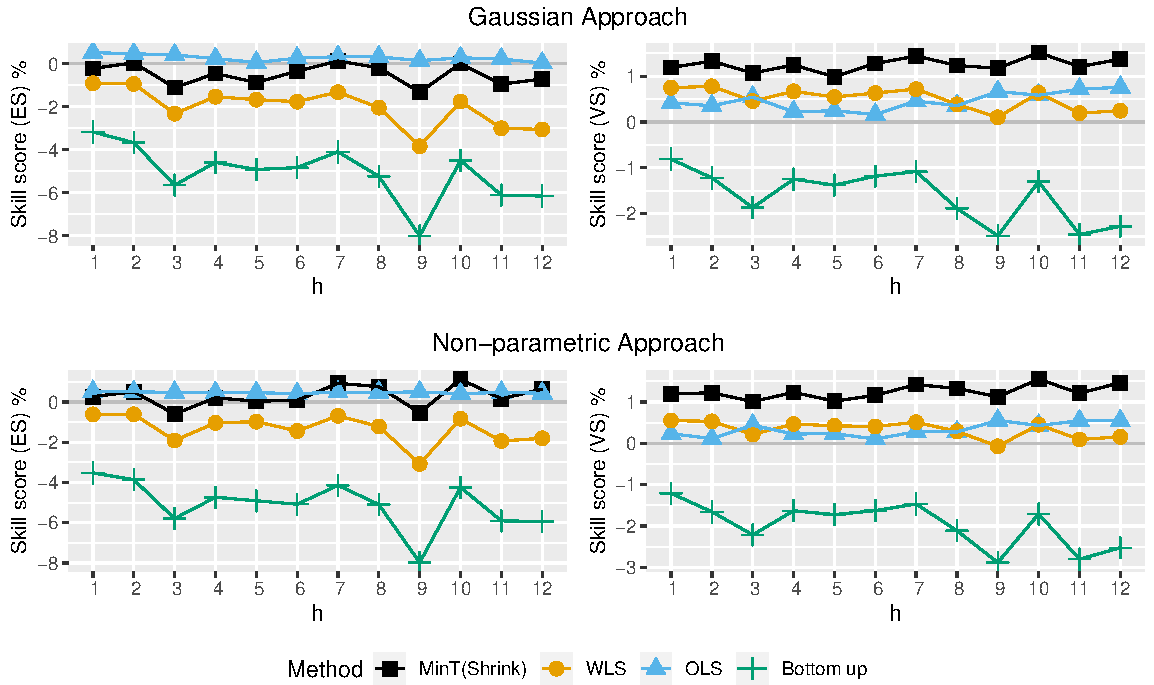
\includegraphics[width= .95\textwidth]{Empirical-results/AllTS_MultiVScores_ETS.pdf}
%	\caption{Skill scores with reference to ETS base forecasts for multivariate predictive distribution of the whole hierarchy from different reconciliation methods are presented. Top panel shows the results from Gaussian approach and the bottom panel shows the results from non-parametric approach. Left and right panels shows the skill scores based on energy score and variogram score respectively.}\label{fig:EmpResults_AllTS_ETS}
%\end{figure}
%
%\begin{figure}[!hbt]
%	\centering
%	\small
%%	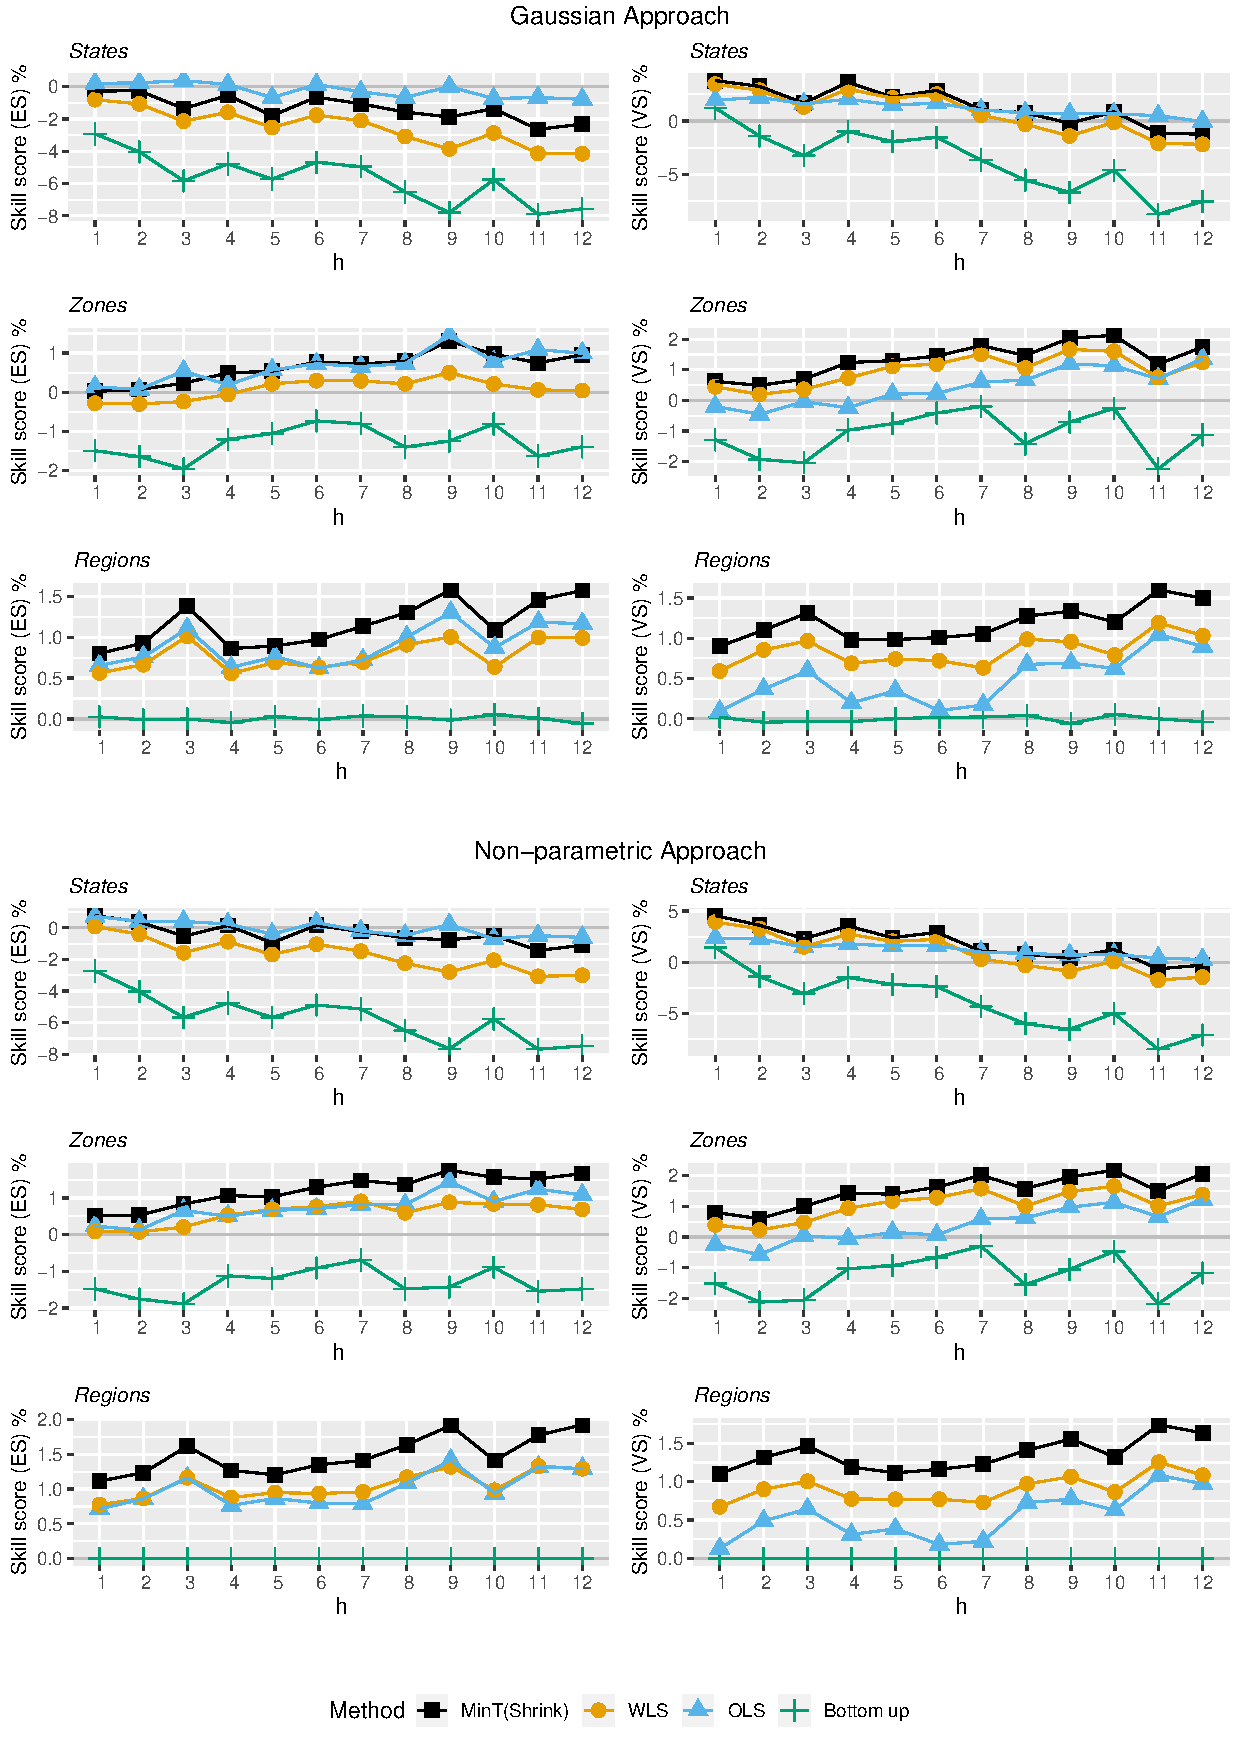
\includegraphics[width= 0.8\textwidth, height= 0.85\textheight]{Empirical-results/Levels_MultiVScores_ETS.pdf}
%	\caption{Skill score (with reference to ETS base forecasts) for multivariate probabilistic forecasts of different levels of the hierarchy are presented. Results from Gaussian approach are presented in the top three panels and results from the non-parametric approach are presented in the bottom three panels.}\label{fig:EmpResults_Levels_ETS}
%\end{figure}
%
%\begin{figure}[!hbt]
%	\centering
%	\small
%%	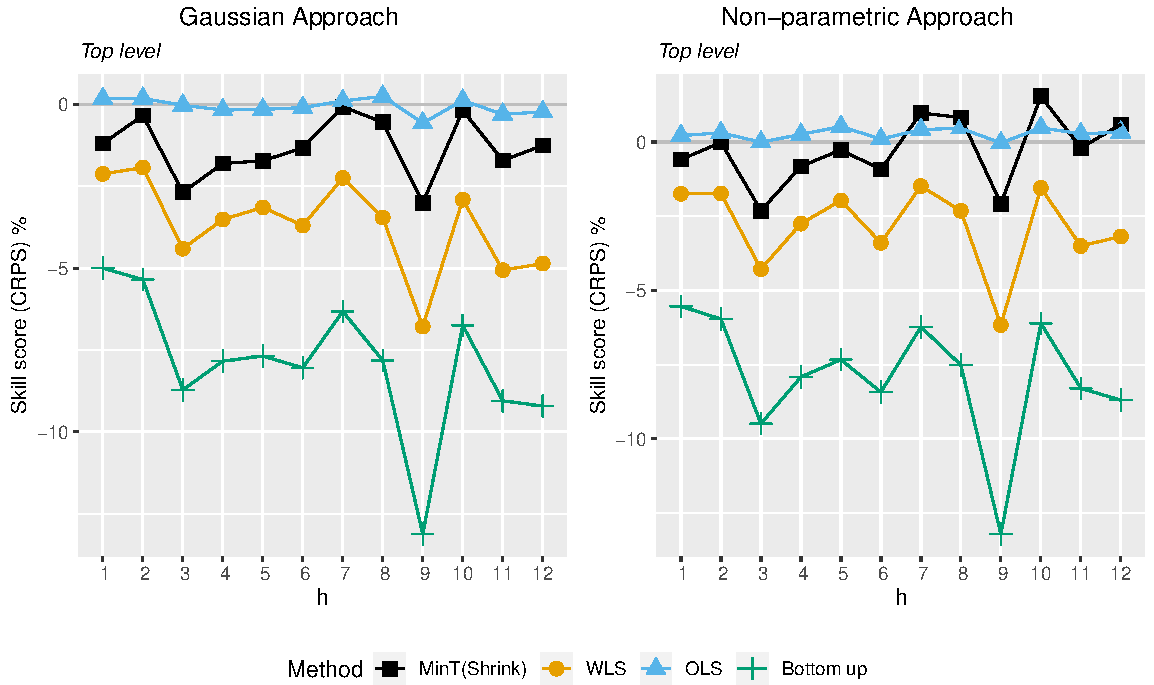
\includegraphics[width= \textwidth]{Empirical-results/UniVScore_TopLevel_ETS.pdf}
%	\caption{Skill score based on CRPS (with reference to the ETS base forecasts) for univariate probabilistic forecasts for the Total (top level) overnight trips are presented. Left panel shows the results from Gaussian approach and right panel shows the results from non-parametric approach. }\label{fig:EmpResults_TopLevel_ETS}
%\end{figure}

\FloatBarrier

\newpage
\subsection{Australian Tourism Data}

\begin{table}[!hb]
	\caption{Geographic hierarchy of Australian tourism flow}\label{table:A1_chap3}
	\centering\tabcolsep=0.08cm
	\fontsize{7}{7}\selectfont
	\resizebox{\linewidth}{!}{
		\begin{tabular}{lllllllllll}
			\toprule
			\multicolumn{3}{c}{\textbf{Level 0 - Total}}    &&  \multicolumn{3}{l}{\textit{Regions cont.}}   &  & \multicolumn{3}{l}{\textit{Regions cont.}} \\
			\cmidrule(lr){1-3}
			1 & {\text{Tot}} & {Australia} &&  37	& AAB & Central Coast && 75  & CBD & Mackay   \\
			\cmidrule(lr){1-3}
			\multicolumn{3}{c}{\textbf{Level 1 - States}} && 38  & ABA & Hunter && 76 & CBE & Capricorn \\
			\cmidrule(lr){1-3}
			2 & A & NSW 				&  & 39  & ABB & North Coast NSW   && 77 & CBF & Gladstone\\
			3 & B & Victoria 			&  & 40  & ACA & South Coast  && 78  & CCA & Whitsundays\\
			4 & C & Queensland 			&  & 41  & ADA & Snowy Mountains && 79  & CCB & Townsville  \\
			5 & D & South Australia     &  & 42  & ADB & Capital Country && 80  & CCC & Tropical North Queensland   \\
			6 & E & Western Australia   &  & 43  & ADC & The Murray   && 81  & CDA & Southern QLD country\\
			7 & F & Tasmania   			&  & 44  & ADD & Riverina  &&82  & CDB & Outback QLD\\
			8 & G & Northern Territory  &  & 45  & AEA & Central NSW &&83  & DAA & Adelaide   \\
			\cmidrule(lr){1-3}
			\multicolumn{3}{c}{\textbf{Level 2 - Zones}}  &  &  46  & AEB & New England North West && 84  & DAB & Barossa\\
			\cmidrule(lr){1-3}
			9 	& AA & Metro NSW 	  	   	&  & 47  & AEC & Outback NSW   &&85  & DAC & Adelaide Hills\\
			10 	& AB & North Coast NSW 	   	&  & 48  & AED & Blue Mountains  && 86  & DBA & Limestone Coast\\
			11	& AC & South Coast NSW	   	&  & 49  & AFA & Canberra   &&  87  & DBB & Fleurieu Peninsula\\
			12	& AD & South NSW 			&  & 50  & BAA & Melbourne &&88  & DBC & Kangaroo Island\\
			13	& AE & North NSW 			&  & 51  & BAB & Peninsula    &&89  & DCA & Murraylands\\
			14	& AF & ACT					&  &  52  & BAC & Geelong  && 90  & DCB & Riverland\\
			15	& BA & Metro VIC			&  &  53  & BBA & Western   &&91  & DCC & Clare Valley\\
			16	& BB & West Coast VIC		&  &  54  & BCA & Lakes  &&92  & DCD & Flinders Range and Outback\\
			17	& BC & East Coast VIC		&  &  55  & BCB & Gippsland    &&93  & DDA & Eyre Peninsula\\
			18	& BD & North East VIC		&  &  56  & BCC & Phillip Island   &&  94  & DDB & Yorke Peninsula \\
			19	& BE & North West VIC		&  &  57  & BDA & Central Murray    &&95  & EAA & Australia's Coral Coast\\
			20  & CA & Metro QLD			&  & 58  & BDB & Goulburn    &&96  & EAB & Experience Perth\\
			21  & CB & Central Coast QLD	&  & 59  & BDC & High Country   &&97  & EAC & Australia's South West\\
			22  & CC & North Coast QLD		&  &  60  & BDD & Melbourne East &&98  & EBA & Australia's North West \\
			23  & CD & Inland QLD			&  &   61  & BDE & Upper Yarra &&99  & ECA & Australia's Golden Outback\\
			24	& DA & Metro SA				&  & 62  & BDF & Murray East  && 100 & FAA & Hobart and South\\
			25	& DB & South Coast SA		&  &  63  & BEA & Wimmera+Mallee &&101 & FBA & East Coast\\
			26	& DC & Inland SA			&  & 64  & BEB & Western Grampians &&102 & FBB & Launceston, Tamar \& North\\
			27	& DD & West Coast SA		&  &65  & BEC & Bendigo Loddon  &&103 & FCA & North West\\
			
			28	& EA & West Coast WA 	& &  66  & BED & Macedon    &&104 & FCB& West coast\\
			29	& EB & North WA			& &  67  & BEE & Spa Country   &&105 & GAA& Darwin \\
			30	& EC & South WA 		& &   68  & BEF & Ballarat     &&106 & GAB& Litchfield Kakadu Arnhem\\
			31	& FA & South TAS		& &  69  & BEG & Central Highlands  &&107 & GAC& Katherine Daly\\
			32	& FB & North East TAS	& & 70  & CAA & Gold Coast  &&108 & GBA& Barkly\\
			33	& FC & North West TAS	& & 71  & CAB & Brisbane  &&109 & GBB& Lasseter\\
			34	& GA & North Coast NT	& & 72  & CAC & Sunshine Coast &&110 & GBC& Alice Springs\\
			35	& GB & Central NT		& &  73  & CBB & Bundaberg      &&111 & GBD& MacDonnell\\
			\cmidrule(lr){1-3}
			\multicolumn{3}{c}{\textbf{Level 2 - Regions}} & & 74  & CBC & Fraser Coast    &&\\
			\cmidrule(lr){1-3}
			36	& AAA & Sydney 			& 	&  &&\\
			
			\bottomrule
		\end{tabular}
	}
\end{table}

\bibliographystyle{agsm}

\bibliography{References_paper2}

\end{document} 